\documentclass{ntuthesis}
%套件安裝處
\usepackage{times}
\usepackage{verbatim}
\usepackage{color}
\usepackage{url}
\usepackage{graphicx}
\usepackage{array}
\usepackage{wallpaper} 
\usepackage{titlesec}
\usepackage{indentfirst}
\usepackage{titletoc}
\usepackage{enumerate}
\usepackage{tikz}
\usepackage{amsmath}
\usepackage{xeCJK}
\usepackage{CJKnumb}
\usepackage{hyperref}
\usepackage{apacite}
\usepackage{multirow}

\defaultCJKfontfeatures{AutoFakeBold=1}
\usetikzlibrary{shapes, arrows}
% Using the tex-text mapping for ligatures etc.
\defaultfontfeatures{Mapping=tex-text}
% Set the default fonts 
\setmainfont{Times New Roman}
\setCJKmainfont{BiauKai}
% Your information goes here
% 存取論文相關資訊
% Syntax: \var{English}{Chinese}
\university{National Taiwan University}{國立臺灣大學}
\college{College of Engineering}{工學院}
\institute{Institute of Industrial Engineering}{工業工程學研究所}
\title{The Research of Parameters Optimization In a Textile Dyeing Process
}{紡織染色製程最佳化問題之研究}
\author{Sheng-Chieh Chen}{陳聖捷}
\studentid{R04546020}
\advisor{I-Hsuan Hong, Ph.D.}{洪一薰 博士}
\defenseyear{2017}{106}
\defensemonth{July}{7}
\defenseday{21}

\begin{document}
\let\cleardoublepage\clearpage
%台大浮水印位置設定
\CenterWallPaper{0.174}{watermark.pdf}
  \setlength{\wpXoffset}{6.1725cm}
  \setlength{\wpYoffset}{10.5225cm}
%封面設定
\frontmatter
\makecover
\titleformat{\chapter}{\centering\Huge\bfseries}{第\,\CJKnumber{\thechapter}\,章}{1em}{}
\titlecontents{chapter}[0em]
{}{\makebox[4.1em][l]
{第\CJKnumber{\thecontentslabel}章}}{}
{\titlerule*[0.7pc]{.}\contentspage}
% \makecertification
% acknowledgements為致謝
%\defaultfont

\BiAppendixChapter{��~~~~л}{Acknowledgement}

\ifxueweidoctor               %��ʿҳü
\fancyhead[CO]{\CJKfamily{song}\xiaowu\leftmark}
\else
\fancyhead[CO]{\CJKfamily{song}\xiaowu ��������ҵ��ѧ\cxueke \cxuewei ѧλ����}
\fi
\fancyhead[CE]{\CJKfamily{song}\xiaowu ��������ҵ��ѧ\cxueke \cxuewei ѧλ���� }%

������ģ����UFO@bbs.hit.edu.cn�ġ���������ҵ��ѧ��ѧ��ʿ��˶ʿ������ģ�塷�Ļ����ϣ�
���ںܶ��˵İ�������ɵģ��ڴ�һ�������DZ�ʾ��л��

�ر��лStanley����������ģ�忪Դ��ĿPluto�Լ���������ģ��Ĵ����޸ģ�
ʹ֮���ӷ��Ϲ�������ģ��Ҫ��

�ر��л�������϶���վ��~Tex~�İ���~Tex��nebula������cucme��
������ʼ���ն�ȫ��֧��ģ�����������Ϊ�����˴����Ĺ�����

��л���괺~(HIT bbs ID: dengnch)�������˴�����ʱ��������ģ���
һϵ�в�����ʹ�ø�~\LaTeX~ģ��Ͷ�Ӧ��~Word~ģ��ĸ�ʽ������ȫһ�¡�

��лˮľ�廪��~\TeX~��~\LaTeX~��ĸ�λ����Ϊ���ṩ�ĸ��ְ�����
�ر���~snoopyzhao~���ѣ���������ĵ�Ϊ��ģ�����������ѣ�ʹ��ģ�����������
˳�����С�

������ĸ�л�������϶���~bbs~վ~Tex~���������ѵĴ���֧�֣�



ֵ���������֮�ʣ������������˽��������ʦ��ͬѧ�����Գ�ֿ��л�⣡

���ȸ�л�ҵĵ�ʦ{\bf ijijij}���ڣ������ĵ��о�����������{\bf
ij}��ʦ����Ľ�����չ���ġ�
����ѧ���ϲ��Ͻ�ȡ������������ִ��׷��ľ�������ѧϰ�İ�����{\bf
ij}��ʦ��������̵���ʶ������dz���Ľ�������������ӡ��


��л{\bf ijijij}���ں�{\bf ijijij}���ڶ���ѧϰ�͹����İ�����
�����ڷܵĹ������硢��۵�����̬�ȶ�����ظ�Ⱦ���ҡ���л{\bf
ijijij}���ں�{\bf ijijij}���ڶ���ѧҵ�������ϵĹ��ġ�


��л��ʿ��{\bf ijijij}��{\bf ijijij}��{\bf ijijij}��{\bf ijijij}��
���ҵ���˽�����ͻ���֧�֡���лʵ�������е��ֵܽ����ǣ�
����Ҷȹ����ⳤ�õ�ѧϰ���о��׶Σ������ҽ�����⣬����˼�롣

����ر�Ҫ��л�ҵ������ǣ����Ƕ���Ҫ�����٣��������ҵĶ��ǹػ���֧�ֺ����⡣


% Abstract
\clearpage
\thispagestyle{plain}
\phantomsection
\addcontentsline{toc}{chapter}{Abstract}

\centerline{\zihao{3}\bfseries Abstract}

\linespread{1.4}\zihao{-4}
\bigskip

This thesis explores the relationship between focus structure and pronoun resolution among non-native speakers of English and French. Firstly we reviewed the existing literature on the mechanism of focus effect and pronoun resolution. Then through a self-paced reading test, we find that focus, in the form of cleft structure does not necessarily increase the salience of a informational unit, thus may not in some cases make it a preferred antecedent for pronoun resolution. This result is line with previous researches on this topic. In our experiment, We also find that focused subject in French and focused object in English are processed faster, but focused subjects in both languages leads to longer response time of anaphora. Furthermore, our research also shows that the congruence between anaphora and focus does not make the latter more accessible. In this regard, we argue that the problem of whether there is subject or object preference in English and French is more complicated than the results of current studies.

\bigskip
\noindent\textbf{\zihao{4} Keywords:} 
focus effect, pronoun resolution, self-paced reading, English, French


\renewcommand\contentsname{目錄}
\tableofcontents
\addcontentsline{toc}{chapter}{\contentsname}

\renewcommand{\figurename}{圖}
\renewcommand\listfigurename{圖目錄}
\newcommand{\loflabel}{圖}
\renewcommand{\numberline}[1]{\loflabel~#1\hspace*{1em}}
\listoffigures
\addcontentsline{toc}{chapter}{\listfigurename}

\renewcommand{\tablename}{表}
\renewcommand\listtablename{表目錄}
\newcommand{\lotlabel}{表}
\renewcommand{\numberline}[1]{\lotlabel~#1\hspace*{1em}}
\listoftables
\addcontentsline{toc}{chapter}{\listtablename}
\mainmatter
\setlength{\parindent}{2em}
% 主要文章位置
% Chapter 1
\chapter{Introduction}\label{chapter:introduction}

\section{Section}
Citation test~\parencite{latex}.

\subsection{Subsection}
See~\autoref{fig:sample}.

\begin{figure}[htsb]
  \centering
  \includegraphics{logos/tum}
  \caption[Example figure]{An example for a figure.}\label{fig:sample}
\end{figure}

\section{Section}

See~\autoref{tab:sample}, \autoref{fig:sample-drawing}, \autoref{fig:sample-plot}, \autoref{fig:sample-listing}.

\begin{table}[htsb]
  \caption[Example table]{An example for a simple table.}\label{tab:sample}
  \centering
  \begin{tabular}{l l l l}
    \toprule
      A & B & C & D \\
    \midrule
      1 & 2 & 1 & 2 \\
      2 & 3 & 2 & 3 \\
    \bottomrule
  \end{tabular}
\end{table}

\begin{figure}[htsb]
  \centering
  % This should probably go into a file in figures/
  \begin{tikzpicture}[node distance=3cm]
    \node (R0) {$R_1$};
    \node (R1) [right of=R0] {$R_2$};
    \node (R2) [below of=R1] {$R_4$};
    \node (R3) [below of=R0] {$R_3$};
    \node (R4) [right of=R1] {$R_5$};

    \path[every node]
      (R0) edge (R1)
      (R0) edge (R3)
      (R3) edge (R2)
      (R2) edge (R1)
      (R1) edge (R4);
  \end{tikzpicture}
  \caption[Example drawing]{An example for a simple drawing.}\label{fig:sample-drawing}
\end{figure}

\begin{figure}[htsb]
  \centering

  \pgfplotstableset{col sep=&, row sep=\\}
  % This should probably go into a file in data/
  \pgfplotstableread{
    a & b    \\
    1 & 1000 \\
    2 & 1500 \\
    3 & 1600 \\
  }\exampleA
  \pgfplotstableread{
    a & b    \\
    1 & 1200 \\
    2 & 800 \\
    3 & 1400 \\
  }\exampleB
  % This should probably go into a file in figures/
  \begin{tikzpicture}
    \begin{axis}[
        ymin=0,
        legend style={legend pos=south east},
        grid,
        thick,
        ylabel=Y,
        xlabel=X
      ]
      \addplot table[x=a, y=b]{\exampleA};
      \addlegendentry{Example A};
      \addplot table[x=a, y=b]{\exampleB};
      \addlegendentry{Example B};
    \end{axis}
  \end{tikzpicture}
  \caption[Example plot]{An example for a simple plot.}\label{fig:sample-plot}
\end{figure}

\begin{figure}[htsb]
  \centering
  \begin{tabular}{c}
  \begin{lstlisting}[language=SQL]
    SELECT * FROM tbl WHERE tbl.str = "str"
  \end{lstlisting}
  \end{tabular}
  \caption[Example listing]{An example for a source code listing.}\label{fig:sample-listing}
\end{figure}

% Chapter 2
%!TEX root = ../thesis.tex
\chapter{文獻探討}
\label{c:literat}
布料的染整加工程序被認定為一個高耗能型產業\dots。
%!TEX root = ../thesis.tex
\section{模型數值化}
\label{c:ch6.1}
在本研究三個主要模型數值化前,本小節將介紹染色過程中的基本參數,但由於品質模型以及穩定度模型參數,從關聯分析中便可得到估計回歸式,故我們主要針對運作成本模型的參數,詳細介紹各個估計參數的數值,如表\ref{tab:table1}所示
\begin{enumerate}[(1)]
	\item \textbf{熱容量及熱傳導係數:}\\由於染液的水占較大的比例,且熱容量會比水還高,估計染液的熱容量以水的熱容量做為下限估計係數,也就是每公斤的水升溫一度所需要4200焦耳的熱量做為估計數值。同時目前在熱散失估計上同樣以水的熱傳導係數做為估計係數,為每分鐘一公尺深的染液下降一度所散失33.6焦耳的熱能做為估計數值。
	\item \textbf{常溫及最高溫:}\\由紡織廠估計一般常溫以25度為準,而最高溫則分為淺色染程及深色染程所需要的溫度,淺色染程中以110度做為最高溫度,而深色染程中以130度做為最高溫度。
	\item \textbf{單位電價:}\\由於台電提供每度的電價會依照所消耗的電量而做不同的調整,但在這裡目前以平均每度3元做為係數下限值的估計,每度電為1000瓦而一焦耳為3600千瓦$\cdot$秒,所以可以得知每焦耳所花費的費用為1/12,000,000元。
	\item \textbf{單位水價及廢水處理單價:}\\在這裡目前以每度水10元的定值設為係數估計,而一度水為1000公斤,故也可以說每公斤的水約為0.01元。而紡織廠也提出每公斤單位水價基本上以每公斤0.011元計算,而廢水處理則以每公斤0.035元的方式計價。
	\item \textbf{第一段及第三段升溫速率:}\\由於限制式內第二階段升溫速率不超過每分鐘上升4.5度,而且在第一階段及第三階段升溫速率有不可過慢,所以目前以每分鐘上升3度為估計速率。
	\item \textbf{機台占用成本:}\\機台占用成本可能根據廠商對於此種儀器在這些時間當中能夠有多少產能,做為估算占用機台時間的成本。由紡織廠提供現場的單位時間占用機台成本,在這裡目前以每分鐘所占用機台時間成本以每分鐘29元做為估計值。
\end{enumerate}
\begin{table}[!htbp]
	\caption{模型參數估計值對照表}
	\center
	\begin{tabular}{ccc}
\hline	
	\textbf{估計項目} & \textbf{估計係數} & \textbf{單位} \\ \hline \hline
	熱容量($S$) & 4200 & $J/{kg\cdot T}$ \\
	常溫($T_L$) & 25 & $^\circ C$ \\
	最高溫度($T_H$) & 110 & $^\circ C$ \\
	第一段及第三段升溫速率($v$) & 3 & $^\circ C/min$ \\
	布重($M$) & 400 & $kg$ \\
	換水成本($K$) & 12 & $times$ \\
	單位電價($C_{1}$) & 1/12000000 & $NTD/J$ \\
	單位水價($C_{2}$) & 0.011 & $NTD/kg$ \\ 
	機台佔用成本($C_{3}$) & 29 & $NTD/min$ \\
	單位廢水成本($c$) & 0.035 & $NTD/kg$ \\
\hline
\end{tabular}
	\label{tab:table1}
\end{table}
\newpage
在表\ref{tab:table1}中的估計參數,與實際情況會根據不同的紡織廠的環境有所不同,再加上表中的參數我們假設電價以及水價不會隨著季節的變動而不同,也就是設定為平均定值,但經由與紡織產業討論後,並不會對模型造成影響;除了運作成本外,還有與紡織產業討論後得到每個參數因子的上下屆值,如表\ref{tab:table2}
\begin{table}
	\caption{染整參數因子上下界值表}
	\center
	\newcommand{\tabincell}[2]{\begin{tabular}{@{}#1@{}}#2\end{tabular}}  
\begin{tabular}{cccccc}
\hline	
	參數範圍 & \tabincell{c}{第一段目標\\溫度($^\circ C$)} & 
	\tabincell{c}{第二段升溫\\速率($^\circ C/min$)} & 
	\tabincell{c}{第三段目標\\溫度($^\circ C$)} & 
	\tabincell{c}{持溫時間\\($min$)} & 
	{浴比值} \\ 
	\hline \hline
	下界值 & 51 & 1.2 & 76 & 11 & 14\\
	上界值 & 61 & 1.8 & 86 & 19 & 26\\
\hline
\end{tabular}
	\label{tab:table2}
\end{table}
其中,分別為$x_A$、$x_B$、$x_C$、$x_D$以及$x_E$的上下界值。
\\ \textbf{運作成本數值最小化模型}\\
從理論上的模型架構以及方法套用,到本章節要討論,當實際的參數帶入理論模型中,是否可以得到比傳統經驗更優的結果,接下來我們會將理論模型數值化,再針對數值化過後的結果進行求解,以及與傳統比較各個模型中的優劣。
將表\ref{tab:table1}代入變數轉換後的運作成本模型,我們以\ref{model:cost}式表示
	\begin{equation}
	\begin{array}{c}
	\min_{x_A,x_B,x_C,x_D,x_E} \{ 820.7+19x_D+232.7x_E+29t+9.7x_Bt \} \\
	51 \leq x_A \leq 61,\\
	1.2 \leq x_B \leq 1.8,\\
	76 \leq x_C \leq 86,\\
	11 \leq x_D \leq 19,\\
	14 \leq x_E \leq 26,\\
	8.3 \leq t \leq 29.2,\\
	x_C-x_A-x_B\cdot t = 0,\\
	0 \leq f_{\Delta E}(x_A,x_B,x_C,x_D,x_E) \leq 0.8,\\
	95 \leq f_{K/S}(x_A,x_B,x_C,x_D,x_E) \leq 105
	\end{array}
	\label{model:cost}
\end{equation}
從上面式子中,可以觀察到運作成本模型的目標函式都為正數,參數因子愈小,則運作成本就愈小,但在限制式中有對品質進行限制,在求解中就不會那麼的直觀了。
\\ \textbf{穩定度數值模型}\\
從染整製程參數關聯性分析,以推估後的$(\Delta E's\ norm)^2$結果帶入回歸模型,我們以\ref{model:robust}式表示
\begin{equation}
	\begin{array}{c}
	\min_{x_A,x_B,x_C,x_D,x_E} \{ 
	(4.87-0.015z_A-0.17x_B-0.038x_C-0.029x_D)^2+\\
	(-0.015x_B+0.00014x_E)^2+(-0.038x_B+0.0027x_E)^2+\\
	(-0.029x_B-0.0011x_E)^2+(-0.45697+0.000148x_A+\\
	0.00271x_C-0.0011x_D+0.011x_E)^2 \} \\
	51 \leq x_A \leq 61,\\
	1.2 \leq x_B \leq 1.8,\\
	76 \leq x_C \leq 86,\\
	11 \leq x_D \leq 19,\\
	14 \leq x_E \leq 26,\\
	0 \leq f_{\Delta E}(x_A,x_B,x_C,x_D,x_E) \leq 0.8,\\
	95 \leq f_{K/S}(x_A,x_B,x_C,x_D,x_E) \leq 105
	\end{array}
	\label{model:robust}
	\hfill
\end{equation}
\textbf{品質數值模型}\\
從染整製程參數關聯性分析,以推估後的$\Delta E$結果帶入回歸模型,我們以\ref{model:deltaE}式表示
\begin{equation}
	\begin{array}{c}
	\min_{x_A,x_B,x_C,x_D,x_E} \{ 2.54 + 4.87x_B - 0.46x_E - 0.015x_Ax_B + \\ 
	0.00015x_Ax_E - 0.038x_Bx_C - 0.029x_Bx_D + 0.0027x_Cx_D - 0.0011x_Dx_E - \\
	0.086x_B^2 + 0.0056x_E^2 \} \\
	51 \leq x_A \leq 61,\\
	1.2 \leq x_B \leq 1.8,\\
	76 \leq x_C \leq 86,\\
	11 \leq x_D \leq 19,\\
	14 \leq x_E \leq 26,\\
	0 \leq f_{\Delta E}(x_A,x_B,x_C,x_D,x_E) \leq 0.8,\\
	95 \leq f_{K/S}(x_A,x_B,x_C,x_D,x_E) \leq 105
	\end{array}
	\label{model:deltaE}
	\hfill
\end{equation}
至於限制式中,兩個主要的品質指標,由估計後得到的$\Delta E$以及$K/S$數值函式分別為$f_{\Delta E}$估計函式
\begin{equation*}
	\begin{split}
	f_{\Delta E}(x_A,x_B,x_C,x_D,x_E)=2.54 + 4.87x_B - 0.46x_E - \\
	0.015x_Ax_B + 0.00015x_Ax_E - 0.038x_Bx_C - 0.029x_Bx_D + \\
	0.0027x_Cx_D - 0.0011x_Dx_E - 0.086x_B^2 + 0.0056x_E^2 
	\end{split}
\end{equation*}
以及$f_{K/S}$估計函式
\begin{equation*}
	\begin{array}{c}
	f_{K/S}(x_A,x_B,x_C,x_D,x_E)=-57.72+4.46x_A-36.52x_B+3.69x_D+3.51x_E+\\
	0.25x_Ax_B-0.042x_Ax_C-0.029x_Ax_D-0.019x_Ax_E+
	0.15x_Bx_C+0.36x_Bx_D+\\
	0.085x_Bx_E-0.022x_Cx_D-0.022x_Cx_E-0.0019x_Dx_E-0.0027x_A^2+\\
	0.82x_B^2+0.018x_C^2-0.026x_D^2-0.025x_E^2 
	\end{array}
\end{equation*}
得到數值化後的模型從\ref{model:cost}式$\sim$ \ref{model:deltaE}式後,在下一小節我們以序列二次規劃法對數值化的模型進行求解。
% %!TEX root = ../thesis.tex
\section{染色製程參數優化技術}
\label{c:ch2.2}

% Chapter 3
% %!TEX root = ../thesis.tex
\chapter{紡織染色製程現況}
\label{c:description}
圖片放置
\begin{figure} 
\centering  
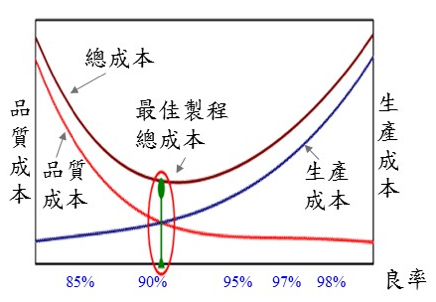
\includegraphics[width=8cm,height=6cm]{Graph/graph1.png}
\caption{染整製程品質成本及生產成本之關係曲線現況描述}
\label{fig:graph1}
\end{figure}
% %!TEX root = ../thesis.tex
\section{模型數值化}
\label{c:ch6.1}
在本研究三個主要模型數值化前,本小節將介紹染色過程中的基本參數,但由於品質模型以及穩定度模型參數,從關聯分析中便可得到估計回歸式,故我們主要針對運作成本模型的參數,詳細介紹各個估計參數的數值,如表\ref{tab:table1}所示
\begin{enumerate}[(1)]
	\item \textbf{熱容量及熱傳導係數:}\\由於染液的水占較大的比例,且熱容量會比水還高,估計染液的熱容量以水的熱容量做為下限估計係數,也就是每公斤的水升溫一度所需要4200焦耳的熱量做為估計數值。同時目前在熱散失估計上同樣以水的熱傳導係數做為估計係數,為每分鐘一公尺深的染液下降一度所散失33.6焦耳的熱能做為估計數值。
	\item \textbf{常溫及最高溫:}\\由紡織廠估計一般常溫以25度為準,而最高溫則分為淺色染程及深色染程所需要的溫度,淺色染程中以110度做為最高溫度,而深色染程中以130度做為最高溫度。
	\item \textbf{單位電價:}\\由於台電提供每度的電價會依照所消耗的電量而做不同的調整,但在這裡目前以平均每度3元做為係數下限值的估計,每度電為1000瓦而一焦耳為3600千瓦$\cdot$秒,所以可以得知每焦耳所花費的費用為1/12,000,000元。
	\item \textbf{單位水價及廢水處理單價:}\\在這裡目前以每度水10元的定值設為係數估計,而一度水為1000公斤,故也可以說每公斤的水約為0.01元。而紡織廠也提出每公斤單位水價基本上以每公斤0.011元計算,而廢水處理則以每公斤0.035元的方式計價。
	\item \textbf{第一段及第三段升溫速率:}\\由於限制式內第二階段升溫速率不超過每分鐘上升4.5度,而且在第一階段及第三階段升溫速率有不可過慢,所以目前以每分鐘上升3度為估計速率。
	\item \textbf{機台占用成本:}\\機台占用成本可能根據廠商對於此種儀器在這些時間當中能夠有多少產能,做為估算占用機台時間的成本。由紡織廠提供現場的單位時間占用機台成本,在這裡目前以每分鐘所占用機台時間成本以每分鐘29元做為估計值。
\end{enumerate}
\begin{table}[!htbp]
	\caption{模型參數估計值對照表}
	\center
	\begin{tabular}{ccc}
\hline	
	\textbf{估計項目} & \textbf{估計係數} & \textbf{單位} \\ \hline \hline
	熱容量($S$) & 4200 & $J/{kg\cdot T}$ \\
	常溫($T_L$) & 25 & $^\circ C$ \\
	最高溫度($T_H$) & 110 & $^\circ C$ \\
	第一段及第三段升溫速率($v$) & 3 & $^\circ C/min$ \\
	布重($M$) & 400 & $kg$ \\
	換水成本($K$) & 12 & $times$ \\
	單位電價($C_{1}$) & 1/12000000 & $NTD/J$ \\
	單位水價($C_{2}$) & 0.011 & $NTD/kg$ \\ 
	機台佔用成本($C_{3}$) & 29 & $NTD/min$ \\
	單位廢水成本($c$) & 0.035 & $NTD/kg$ \\
\hline
\end{tabular}
	\label{tab:table1}
\end{table}
\newpage
在表\ref{tab:table1}中的估計參數,與實際情況會根據不同的紡織廠的環境有所不同,再加上表中的參數我們假設電價以及水價不會隨著季節的變動而不同,也就是設定為平均定值,但經由與紡織產業討論後,並不會對模型造成影響;除了運作成本外,還有與紡織產業討論後得到每個參數因子的上下屆值,如表\ref{tab:table2}
\begin{table}
	\caption{染整參數因子上下界值表}
	\center
	\newcommand{\tabincell}[2]{\begin{tabular}{@{}#1@{}}#2\end{tabular}}  
\begin{tabular}{cccccc}
\hline	
	參數範圍 & \tabincell{c}{第一段目標\\溫度($^\circ C$)} & 
	\tabincell{c}{第二段升溫\\速率($^\circ C/min$)} & 
	\tabincell{c}{第三段目標\\溫度($^\circ C$)} & 
	\tabincell{c}{持溫時間\\($min$)} & 
	{浴比值} \\ 
	\hline \hline
	下界值 & 51 & 1.2 & 76 & 11 & 14\\
	上界值 & 61 & 1.8 & 86 & 19 & 26\\
\hline
\end{tabular}
	\label{tab:table2}
\end{table}
其中,分別為$x_A$、$x_B$、$x_C$、$x_D$以及$x_E$的上下界值。
\\ \textbf{運作成本數值最小化模型}\\
從理論上的模型架構以及方法套用,到本章節要討論,當實際的參數帶入理論模型中,是否可以得到比傳統經驗更優的結果,接下來我們會將理論模型數值化,再針對數值化過後的結果進行求解,以及與傳統比較各個模型中的優劣。
將表\ref{tab:table1}代入變數轉換後的運作成本模型,我們以\ref{model:cost}式表示
	\begin{equation}
	\begin{array}{c}
	\min_{x_A,x_B,x_C,x_D,x_E} \{ 820.7+19x_D+232.7x_E+29t+9.7x_Bt \} \\
	51 \leq x_A \leq 61,\\
	1.2 \leq x_B \leq 1.8,\\
	76 \leq x_C \leq 86,\\
	11 \leq x_D \leq 19,\\
	14 \leq x_E \leq 26,\\
	8.3 \leq t \leq 29.2,\\
	x_C-x_A-x_B\cdot t = 0,\\
	0 \leq f_{\Delta E}(x_A,x_B,x_C,x_D,x_E) \leq 0.8,\\
	95 \leq f_{K/S}(x_A,x_B,x_C,x_D,x_E) \leq 105
	\end{array}
	\label{model:cost}
\end{equation}
從上面式子中,可以觀察到運作成本模型的目標函式都為正數,參數因子愈小,則運作成本就愈小,但在限制式中有對品質進行限制,在求解中就不會那麼的直觀了。
\\ \textbf{穩定度數值模型}\\
從染整製程參數關聯性分析,以推估後的$(\Delta E's\ norm)^2$結果帶入回歸模型,我們以\ref{model:robust}式表示
\begin{equation}
	\begin{array}{c}
	\min_{x_A,x_B,x_C,x_D,x_E} \{ 
	(4.87-0.015z_A-0.17x_B-0.038x_C-0.029x_D)^2+\\
	(-0.015x_B+0.00014x_E)^2+(-0.038x_B+0.0027x_E)^2+\\
	(-0.029x_B-0.0011x_E)^2+(-0.45697+0.000148x_A+\\
	0.00271x_C-0.0011x_D+0.011x_E)^2 \} \\
	51 \leq x_A \leq 61,\\
	1.2 \leq x_B \leq 1.8,\\
	76 \leq x_C \leq 86,\\
	11 \leq x_D \leq 19,\\
	14 \leq x_E \leq 26,\\
	0 \leq f_{\Delta E}(x_A,x_B,x_C,x_D,x_E) \leq 0.8,\\
	95 \leq f_{K/S}(x_A,x_B,x_C,x_D,x_E) \leq 105
	\end{array}
	\label{model:robust}
	\hfill
\end{equation}
\textbf{品質數值模型}\\
從染整製程參數關聯性分析,以推估後的$\Delta E$結果帶入回歸模型,我們以\ref{model:deltaE}式表示
\begin{equation}
	\begin{array}{c}
	\min_{x_A,x_B,x_C,x_D,x_E} \{ 2.54 + 4.87x_B - 0.46x_E - 0.015x_Ax_B + \\ 
	0.00015x_Ax_E - 0.038x_Bx_C - 0.029x_Bx_D + 0.0027x_Cx_D - 0.0011x_Dx_E - \\
	0.086x_B^2 + 0.0056x_E^2 \} \\
	51 \leq x_A \leq 61,\\
	1.2 \leq x_B \leq 1.8,\\
	76 \leq x_C \leq 86,\\
	11 \leq x_D \leq 19,\\
	14 \leq x_E \leq 26,\\
	0 \leq f_{\Delta E}(x_A,x_B,x_C,x_D,x_E) \leq 0.8,\\
	95 \leq f_{K/S}(x_A,x_B,x_C,x_D,x_E) \leq 105
	\end{array}
	\label{model:deltaE}
	\hfill
\end{equation}
至於限制式中,兩個主要的品質指標,由估計後得到的$\Delta E$以及$K/S$數值函式分別為$f_{\Delta E}$估計函式
\begin{equation*}
	\begin{split}
	f_{\Delta E}(x_A,x_B,x_C,x_D,x_E)=2.54 + 4.87x_B - 0.46x_E - \\
	0.015x_Ax_B + 0.00015x_Ax_E - 0.038x_Bx_C - 0.029x_Bx_D + \\
	0.0027x_Cx_D - 0.0011x_Dx_E - 0.086x_B^2 + 0.0056x_E^2 
	\end{split}
\end{equation*}
以及$f_{K/S}$估計函式
\begin{equation*}
	\begin{array}{c}
	f_{K/S}(x_A,x_B,x_C,x_D,x_E)=-57.72+4.46x_A-36.52x_B+3.69x_D+3.51x_E+\\
	0.25x_Ax_B-0.042x_Ax_C-0.029x_Ax_D-0.019x_Ax_E+
	0.15x_Bx_C+0.36x_Bx_D+\\
	0.085x_Bx_E-0.022x_Cx_D-0.022x_Cx_E-0.0019x_Dx_E-0.0027x_A^2+\\
	0.82x_B^2+0.018x_C^2-0.026x_D^2-0.025x_E^2 
	\end{array}
\end{equation*}
得到數值化後的模型從\ref{model:cost}式$\sim$ \ref{model:deltaE}式後,在下一小節我們以序列二次規劃法對數值化的模型進行求解。
% %!TEX root = ../thesis.tex
\section{染色製程參數優化技術}
\label{c:ch2.2}

% Chapter 4
%!TEX root = ../thesis.tex
\chapter{染整製程模型建立}
\label{c:model}
前面章節敘述了介紹了文獻探討以及染整產業的現況,目前業者對於染整製程優化的部分以直觀的方法比較,學術上則是以啟發式演算法進行求解,如基因演算法\cite{Wu.etc},目前較少以非線性規劃的方法求解,故本章節主要詳細介紹如何建構染整製程最佳化模型。
%!TEX root = ../thesis.tex
\section{模型數值化}
\label{c:ch6.1}
在本研究三個主要模型數值化前,本小節將介紹染色過程中的基本參數,但由於品質模型以及穩定度模型參數,從關聯分析中便可得到估計回歸式,故我們主要針對運作成本模型的參數,詳細介紹各個估計參數的數值,如表\ref{tab:table1}所示
\begin{enumerate}[(1)]
	\item \textbf{熱容量及熱傳導係數:}\\由於染液的水占較大的比例,且熱容量會比水還高,估計染液的熱容量以水的熱容量做為下限估計係數,也就是每公斤的水升溫一度所需要4200焦耳的熱量做為估計數值。同時目前在熱散失估計上同樣以水的熱傳導係數做為估計係數,為每分鐘一公尺深的染液下降一度所散失33.6焦耳的熱能做為估計數值。
	\item \textbf{常溫及最高溫:}\\由紡織廠估計一般常溫以25度為準,而最高溫則分為淺色染程及深色染程所需要的溫度,淺色染程中以110度做為最高溫度,而深色染程中以130度做為最高溫度。
	\item \textbf{單位電價:}\\由於台電提供每度的電價會依照所消耗的電量而做不同的調整,但在這裡目前以平均每度3元做為係數下限值的估計,每度電為1000瓦而一焦耳為3600千瓦$\cdot$秒,所以可以得知每焦耳所花費的費用為1/12,000,000元。
	\item \textbf{單位水價及廢水處理單價:}\\在這裡目前以每度水10元的定值設為係數估計,而一度水為1000公斤,故也可以說每公斤的水約為0.01元。而紡織廠也提出每公斤單位水價基本上以每公斤0.011元計算,而廢水處理則以每公斤0.035元的方式計價。
	\item \textbf{第一段及第三段升溫速率:}\\由於限制式內第二階段升溫速率不超過每分鐘上升4.5度,而且在第一階段及第三階段升溫速率有不可過慢,所以目前以每分鐘上升3度為估計速率。
	\item \textbf{機台占用成本:}\\機台占用成本可能根據廠商對於此種儀器在這些時間當中能夠有多少產能,做為估算占用機台時間的成本。由紡織廠提供現場的單位時間占用機台成本,在這裡目前以每分鐘所占用機台時間成本以每分鐘29元做為估計值。
\end{enumerate}
\begin{table}[!htbp]
	\caption{模型參數估計值對照表}
	\center
	\begin{tabular}{ccc}
\hline	
	\textbf{估計項目} & \textbf{估計係數} & \textbf{單位} \\ \hline \hline
	熱容量($S$) & 4200 & $J/{kg\cdot T}$ \\
	常溫($T_L$) & 25 & $^\circ C$ \\
	最高溫度($T_H$) & 110 & $^\circ C$ \\
	第一段及第三段升溫速率($v$) & 3 & $^\circ C/min$ \\
	布重($M$) & 400 & $kg$ \\
	換水成本($K$) & 12 & $times$ \\
	單位電價($C_{1}$) & 1/12000000 & $NTD/J$ \\
	單位水價($C_{2}$) & 0.011 & $NTD/kg$ \\ 
	機台佔用成本($C_{3}$) & 29 & $NTD/min$ \\
	單位廢水成本($c$) & 0.035 & $NTD/kg$ \\
\hline
\end{tabular}
	\label{tab:table1}
\end{table}
\newpage
在表\ref{tab:table1}中的估計參數,與實際情況會根據不同的紡織廠的環境有所不同,再加上表中的參數我們假設電價以及水價不會隨著季節的變動而不同,也就是設定為平均定值,但經由與紡織產業討論後,並不會對模型造成影響;除了運作成本外,還有與紡織產業討論後得到每個參數因子的上下屆值,如表\ref{tab:table2}
\begin{table}
	\caption{染整參數因子上下界值表}
	\center
	\newcommand{\tabincell}[2]{\begin{tabular}{@{}#1@{}}#2\end{tabular}}  
\begin{tabular}{cccccc}
\hline	
	參數範圍 & \tabincell{c}{第一段目標\\溫度($^\circ C$)} & 
	\tabincell{c}{第二段升溫\\速率($^\circ C/min$)} & 
	\tabincell{c}{第三段目標\\溫度($^\circ C$)} & 
	\tabincell{c}{持溫時間\\($min$)} & 
	{浴比值} \\ 
	\hline \hline
	下界值 & 51 & 1.2 & 76 & 11 & 14\\
	上界值 & 61 & 1.8 & 86 & 19 & 26\\
\hline
\end{tabular}
	\label{tab:table2}
\end{table}
其中,分別為$x_A$、$x_B$、$x_C$、$x_D$以及$x_E$的上下界值。
\\ \textbf{運作成本數值最小化模型}\\
從理論上的模型架構以及方法套用,到本章節要討論,當實際的參數帶入理論模型中,是否可以得到比傳統經驗更優的結果,接下來我們會將理論模型數值化,再針對數值化過後的結果進行求解,以及與傳統比較各個模型中的優劣。
將表\ref{tab:table1}代入變數轉換後的運作成本模型,我們以\ref{model:cost}式表示
	\begin{equation}
	\begin{array}{c}
	\min_{x_A,x_B,x_C,x_D,x_E} \{ 820.7+19x_D+232.7x_E+29t+9.7x_Bt \} \\
	51 \leq x_A \leq 61,\\
	1.2 \leq x_B \leq 1.8,\\
	76 \leq x_C \leq 86,\\
	11 \leq x_D \leq 19,\\
	14 \leq x_E \leq 26,\\
	8.3 \leq t \leq 29.2,\\
	x_C-x_A-x_B\cdot t = 0,\\
	0 \leq f_{\Delta E}(x_A,x_B,x_C,x_D,x_E) \leq 0.8,\\
	95 \leq f_{K/S}(x_A,x_B,x_C,x_D,x_E) \leq 105
	\end{array}
	\label{model:cost}
\end{equation}
從上面式子中,可以觀察到運作成本模型的目標函式都為正數,參數因子愈小,則運作成本就愈小,但在限制式中有對品質進行限制,在求解中就不會那麼的直觀了。
\\ \textbf{穩定度數值模型}\\
從染整製程參數關聯性分析,以推估後的$(\Delta E's\ norm)^2$結果帶入回歸模型,我們以\ref{model:robust}式表示
\begin{equation}
	\begin{array}{c}
	\min_{x_A,x_B,x_C,x_D,x_E} \{ 
	(4.87-0.015z_A-0.17x_B-0.038x_C-0.029x_D)^2+\\
	(-0.015x_B+0.00014x_E)^2+(-0.038x_B+0.0027x_E)^2+\\
	(-0.029x_B-0.0011x_E)^2+(-0.45697+0.000148x_A+\\
	0.00271x_C-0.0011x_D+0.011x_E)^2 \} \\
	51 \leq x_A \leq 61,\\
	1.2 \leq x_B \leq 1.8,\\
	76 \leq x_C \leq 86,\\
	11 \leq x_D \leq 19,\\
	14 \leq x_E \leq 26,\\
	0 \leq f_{\Delta E}(x_A,x_B,x_C,x_D,x_E) \leq 0.8,\\
	95 \leq f_{K/S}(x_A,x_B,x_C,x_D,x_E) \leq 105
	\end{array}
	\label{model:robust}
	\hfill
\end{equation}
\textbf{品質數值模型}\\
從染整製程參數關聯性分析,以推估後的$\Delta E$結果帶入回歸模型,我們以\ref{model:deltaE}式表示
\begin{equation}
	\begin{array}{c}
	\min_{x_A,x_B,x_C,x_D,x_E} \{ 2.54 + 4.87x_B - 0.46x_E - 0.015x_Ax_B + \\ 
	0.00015x_Ax_E - 0.038x_Bx_C - 0.029x_Bx_D + 0.0027x_Cx_D - 0.0011x_Dx_E - \\
	0.086x_B^2 + 0.0056x_E^2 \} \\
	51 \leq x_A \leq 61,\\
	1.2 \leq x_B \leq 1.8,\\
	76 \leq x_C \leq 86,\\
	11 \leq x_D \leq 19,\\
	14 \leq x_E \leq 26,\\
	0 \leq f_{\Delta E}(x_A,x_B,x_C,x_D,x_E) \leq 0.8,\\
	95 \leq f_{K/S}(x_A,x_B,x_C,x_D,x_E) \leq 105
	\end{array}
	\label{model:deltaE}
	\hfill
\end{equation}
至於限制式中,兩個主要的品質指標,由估計後得到的$\Delta E$以及$K/S$數值函式分別為$f_{\Delta E}$估計函式
\begin{equation*}
	\begin{split}
	f_{\Delta E}(x_A,x_B,x_C,x_D,x_E)=2.54 + 4.87x_B - 0.46x_E - \\
	0.015x_Ax_B + 0.00015x_Ax_E - 0.038x_Bx_C - 0.029x_Bx_D + \\
	0.0027x_Cx_D - 0.0011x_Dx_E - 0.086x_B^2 + 0.0056x_E^2 
	\end{split}
\end{equation*}
以及$f_{K/S}$估計函式
\begin{equation*}
	\begin{array}{c}
	f_{K/S}(x_A,x_B,x_C,x_D,x_E)=-57.72+4.46x_A-36.52x_B+3.69x_D+3.51x_E+\\
	0.25x_Ax_B-0.042x_Ax_C-0.029x_Ax_D-0.019x_Ax_E+
	0.15x_Bx_C+0.36x_Bx_D+\\
	0.085x_Bx_E-0.022x_Cx_D-0.022x_Cx_E-0.0019x_Dx_E-0.0027x_A^2+\\
	0.82x_B^2+0.018x_C^2-0.026x_D^2-0.025x_E^2 
	\end{array}
\end{equation*}
得到數值化後的模型從\ref{model:cost}式$\sim$ \ref{model:deltaE}式後,在下一小節我們以序列二次規劃法對數值化的模型進行求解。
%!TEX root = ../thesis.tex
\section{染色製程參數優化技術}
\label{c:ch2.2}

%!TEX root = ../thesis.tex
\section{染整製程模型求解}
\label{c:ch5.3}
在上一小節當中,我們介紹了本研究的求解方法,而在本小節當中我們會序列二次規劃法套用到本研究主要三個模型當中,並根據圖3.3的序列二次規劃演算流程,搜尋此三個模型的最佳染整參數組合。
\\\textbf{運作成本最小化模型}

在進行演算流程前,我們先將模型進行轉化以及整理,由3.16式當中,首先我們藉由增加鬆弛變數(slack variable) $w_{ij}$將不等式型態轉為等式的型態$h_{i}(x)$,在第一行到第五行不等式中,將其轉換為
\begin{equation}
	\begin{array}{c}
	x_{i}-i_{upper}-w_{i0}=0,\\
	i_{lower}-x{i}-w_{i1}=0,\\
	i\in \{A,B,C,D,E\}
	\end{array}
\label{eq:hx1}
\end{equation}
由 \ref{eq:hx1} 式中我們從 \ref{eq:constraint2} 式中的前五行不等式的轉換下,我們得到$h_{1}(x) \sim h_{10}(x)$,在 \ref{eq:constraint2} 式的第六行不等式,我們將其轉換為 \ref{eq:hxt} 式而得到$h_{11}(x) \sim h_{12}(x)$
\begin{equation}
	\begin{array}{c}
	t-(C_{upper}-A_{lower})/B_{lower}-w_{t0}=0,\\
	(C_{lower}-A_{upper})/B_{upper}-t-w_{t1}=0
	\end{array}
\label{eq:hxt}
\end{equation}
而第七行則為$h_{13}(x)=x_C-x_A-x_B\cdot t$,最後把 \ref{eq:deltaEf} 及 \ref{eq:KSf}式帶入 \ref{eq:constraint2} 式中轉換,並得到$h_{14}(x) \sim h_{17}(x)$,如 \ref{eq:hx2} 式
\begin{equation}
	\begin{array}{c}
	\sum_i C_i\cdot x_i + \sum_i C_{ii}\cdot x_i^2+\sum_i\sum_j C_{ij}\cdot x_{i}\cdot x_{j}-\Delta E_{upper}-w_{\Delta E0}=0,\\
	\Delta E_{lower}-\sum_i C_i\cdot x_i + \sum_i C_{ii}\cdot x_i^2+\sum_i\sum_j C_{ij}\cdot x_{i}\cdot x_{j}-w_{\Delta E1}=0,\\
	\sum_i C_i^{'}\cdot x_i+ \sum_i C_{ii}^{'}\cdot x_i^2+\sum_i\sum_j C_{ij}^{'}\cdot x_{i}\cdot x_{j}-K/S_{upper}-w_{K/S0}=0,\\
	K/S_{lower}-\sum_i C_i^{'}\cdot x_i+ \sum_i C_{ii}^{'}\cdot x_i^2+\sum_i\sum_j C_{ij}^{'}\cdot x_{i}\cdot x_{j}-w_{K/S1}=0,\\
	i,j\in \{A,B,C,D,E\} , i\neq j
	\end{array}
\label{eq:hx2}
\end{equation}
因此我們可以從 \ref{eq:cost2} 式與上面轉換後的限制式合併後,得到 \ref{eq:cost3} 式
\begin{equation}
	\begin{split}
	L(x,t,\lambda)=[C_1SM(T_H-T_L)+(C_2+c)MK]\cdot x_E+\\
	C_3 \cdot [t\cdot (v-x_B) +(T_H-T_L)/v+x_D]-\sum_{i=1}^{17} \lambda_{i}\cdot h_{i}(x)
	\end{split}
\label{eq:cost3}
\end{equation}
並從 \ref{eq:cost3} 式推得$\bigtriangledown L(x,t,\lambda)$,如 \ref{eq:costg}式
\begin{equation}
\bigtriangledown L(x,\lambda)=\left[ 
	\begin{array}{c}
	\lambda_{2}-\lambda_{1}-(\lambda_{14}-\lambda_{15}) \frac{\partial f_{\Delta E}}{\partial x_{A}}-(\lambda_{16}-\lambda_{17}) \frac{\partial f_{K/S}}{\partial x_{A}} \\

	\lambda_{4}-\lambda_{3}-(\lambda_{14}-\lambda_{15}) \frac{\partial f_{\Delta E}}{\partial x_{B}}-(\lambda_{16}-\lambda_{17}) \frac{\partial f_{K/S}}{\partial x_{B}}+C_{3} \Delta T t/v \\

	\lambda_{6}-\lambda_{5}-(\lambda_{14}-\lambda_{15}) \frac{\partial f_{\Delta E}}{\partial x_{C}}-(\lambda_{16}-\lambda_{17}) \frac{\partial f_{K/S}}{\partial x_{C}} \\

	C_{3}+\lambda_{8}-\lambda_{7}-(\lambda_{14}-\lambda_{15}) \frac{\partial f_{\Delta E}}{\partial x_{D}}-(\lambda_{16}-\lambda_{17}) \frac{\partial f_{K/S}}{\partial x_{D}} \\

	Const+\lambda_{10}-\lambda_{9}-(\lambda_{14}-\lambda_{15}) \frac{\partial f_{\Delta E}}{\partial x_{E}}-(\lambda_{16}-\lambda_{17}) \frac{\partial f_{K/S}}{\partial x_{E}} \\

	\end{array}
	\right]
\label{eq:costg}
\end{equation}
其中$Const=[C_1SM(T_H-T_L)+(C_2+c)MK]$以及$\Delta T=(T_{H}-T_{L})$,而$\Delta E$和$K/S$估計式的偏微分分別為\\
\begin{equation*}
	\begin{array}{c}
		\frac{\partial f_{\Delta E}}{\partial x_{i}}=C_{i}+2C_{ii}x_{i}+(\sum_{i} C_{iA} x_{i}+\sum_{j} c_{Aj} x_{j}) \\
		\frac{\partial f_{K/S}}{\partial x_{i}}=C_{i}^{'}+2C_{ii}^{'}x_{i}+(\sum_{i} C_{iA}^{'} x_{i}+\sum_{j} c_{Aj}^{'} x_{j})\\
		i,j\in {A,B,C,D,E}
	\end{array}
\end{equation*}
再將$\bigtriangledown L(x,\lambda)$以及$h_{1}(x)\sim h_{17}(x)$得到$\Psi(x,\lambda)$以及$J(x,\lambda)$。
\\\textbf{穩健度模型}

在穩健度模型中,我們同樣先將模型進行轉化以及整理,由 \ref{eq:constraint} 式當中,首先我們藉由增加鬆弛變數$w_{ij}$將不等式型態轉為等式的型態$h_{i}(x)$,在第一行到第五行不等式中,與 \ref{eq:hx1} 式相同,便可得到$h_{1}(x) \sim h_{10}(x)$,最後把 \ref{eq:deltaEf} 及 \ref{eq:KSf} 帶入 \ref{eq:constraint} 式中轉換,並得到$h_{11}(x) \sim h_{14}(x)$,與 \ref{eq:hx2} 式相同,因此我們可以從 \ref{eq:robust2} 式與上面轉換後的限制式合併後,得到 \ref{eq:robust3} 式
\begin{equation}
	\begin{split}
	L(x,\lambda)=\sum_{i}[C_{i}+2C_{ii}\cdot x_i+\sum_j(C_{ij}+C_{ji})\cdot x_i]^{2}-\sum_{i=1}^{14} \lambda_{i}\cdot h_{i}(x)
	\end{split}
\label{eq:robust3}
\end{equation}
並從 \ref{eq:robust3} 式推得$\bigtriangledown L(x,t,\lambda)$,如 \ref{eq:robustg} 式 \newpage
\begin{equation}
\bigtriangledown L(x,\lambda)=\left[ 
	\begin{array}{c}
	\lambda_{2}-\lambda_{1}-(\lambda_{14}-\lambda_{15}+Const_{A}) \frac{\partial f_{\Delta E}}{\partial x_{A}}-(\lambda_{16}-\lambda_{17}) \frac{\partial f_{K/S}}{\partial x_{A}} \\

	\lambda_{4}-\lambda_{3}-(\lambda_{14}-\lambda_{15}+Const_{B}) \frac{\partial f_{\Delta E}}{\partial x_{B}}-(\lambda_{16}-\lambda_{17}) \frac{\partial f_{K/S}}{\partial x_{B}} \\

	\lambda_{6}-\lambda_{5}-(\lambda_{14}-\lambda_{15}+Const_{C}) \frac{\partial f_{\Delta E}}{\partial x_{C}}-(\lambda_{16}-\lambda_{17}) \frac{\partial f_{K/S}}{\partial x_{C}} \\

	\lambda_{8}-\lambda_{7}-(\lambda_{14}-\lambda_{15}+Const_{D}) \frac{\partial f_{\Delta E}}{\partial x_{D}}-(\lambda_{16}-\lambda_{17}) \frac{\partial f_{K/S}}{\partial x_{D}} \\

	\lambda_{10}-\lambda_{9}-(\lambda_{14}-\lambda_{15}+Const_{E}) \frac{\partial f_{\Delta E}}{\partial x_{E}}-(\lambda_{16}-\lambda_{17}) \frac{\partial f_{K/S}}{\partial x_{E}} 
	\end{array}
	\right]
\label{eq:robustg}
\end{equation}
其中$Const_{i}=4C_{ii}$而$i\in \{A,B,C,D,E\}$,再將$\bigtriangledown L(x,\lambda)$以及$h_{1}(x)\sim h_{14}(x)$得到$\Psi(x,\lambda)$以及$J(x,\lambda)$。
\\\textbf{品質模型($\Delta E$模型)}

品質模型($\Delta E$模型)中,我們同樣先將模型進行轉化以及整理,由 \ref{eq:constraint} 式當中,首先我們藉由增加鬆弛變數$w_{ij}$將不等式型態轉為等式的型態$h_{i}(x)$,在第一行到第五行不等式中,與 \ref{eq:hx1} 式相同,便可得到$h_{1}(x) \sim h_{10}(x)$,最後把 \ref{eq:deltaEf} 及 \ref{eq:KSf} 帶入 \ref{eq:constraint} 式中轉換,並得到$h_{11}(x) \sim h_{14}(x)$,與 \ref{eq:hx2} 式相同,因此我們可以從 \ref{eq:deltaE2} 式與上面轉換後的限制式合併後,得到 \ref{eq:deltaE3} 式
\begin{equation}
	\begin{split}
	L(x,\lambda)=\sum_i C_i\cdot x_i + \sum_i C_{ii}\cdot x_i^2+\sum_i\sum_j C_{ij}\cdot x_{i}\cdot x_{j}-\sum_{i=1}^{14} \lambda_{i}\cdot h_{i}(x)
	\end{split}
\label{eq:deltaE3}
\end{equation}
並從 \ref{eq:deltaE3} 式推得$\bigtriangledown L(x,t,\lambda)$,如 \ref{eq:deltaEg} 式
\begin{equation}
\bigtriangledown L(x,\lambda)=\left[ 
	\begin{array}{c}
	\lambda_{2}-\lambda_{1}-(\lambda_{14}-\lambda_{15}+Const_{A}) \frac{\partial f_{\Delta E}}{\partial x_{A}}-(\lambda_{16}-\lambda_{17}) \frac{\partial f_{K/S}}{\partial x_{A}} \\

	\lambda_{4}-\lambda_{3}-(\lambda_{14}-\lambda_{15}+Const_{B}) \frac{\partial f_{\Delta E}}{\partial x_{B}}-(\lambda_{16}-\lambda_{17}) \frac{\partial f_{K/S}}{\partial x_{B}} \\

	\lambda_{6}-\lambda_{5}-(\lambda_{14}-\lambda_{15}+Const_{C}) \frac{\partial f_{\Delta E}}{\partial x_{C}}-(\lambda_{16}-\lambda_{17}) \frac{\partial f_{K/S}}{\partial x_{C}} \\

	\lambda_{8}-\lambda_{7}-(\lambda_{14}-\lambda_{15}+Const_{D}) \frac{\partial f_{\Delta E}}{\partial x_{D}}-(\lambda_{16}-\lambda_{17}) \frac{\partial f_{K/S}}{\partial x_{D}} \\

	\lambda_{10}-\lambda_{9}-(\lambda_{14}-\lambda_{15}+Const_{E}) \frac{\partial f_{\Delta E}}{\partial x_{E}}-(\lambda_{16}-\lambda_{17}) \frac{\partial f_{K/S}}{\partial x_{E}} 
	\end{array}
	\right]
\label{eq:deltaEg}
\end{equation}
其中$Const_{i}=C_{i}+2C_{ii}x_{i}+\sum_{j} (C_{ij}+C_{ji})x_{j}$而$i,j\in \{A,B,C,D,E\},i\neq j$,再將$\bigtriangledown L(x,\lambda)$以及$h_{1}(x)\sim h_{14}(x)$得到$\Psi(x,\lambda)$以及$J(x,\lambda)$。

我們從三個染整製程模型進行計算後,我們開始圖 \ref{fig:flow3} 的演算步驟搜尋運作成本模型的最佳解。在給定初始值的步驟當中,雖然序列二次規劃對於初始解的選擇可以不限於可行解當中,但在本研究會根據紡織廠所限定的可行解範圍內隨機挑選,\cite{Nocedal.etc}也表示,由於序列二次規劃法在估計原模型問題時好的起始解對於好的起始解對於結果來說,也會比較精確,故起始組合$x_{0}$從經驗上選取一組較為常用的解作為起始組合,而起始的Lagrange乘數$\lambda_{0}$我們則根據KKT條件下,我們以
\begin{equation*}
\lambda^{0}=-[\bigtriangledown h(x^{0})^{T}\bigtriangledown h(x^{0})]^{-1}\bigtriangledown h(x^{0})^{T}\bigtriangledown f(x^{0})
\end{equation*}
作為乘數的起始值,此外我們還需要設定迭代停止的依據,本研究以$x^{k+1}-x^{k}\leq \epsilon$作為演算終止的依據,而$\epsilon$在這裡我們設定在$10^{-5}$,而起始估計矩陣$B_{0}$通常則以單位矩陣作為起始的估計矩陣,確定各個起始值後,我們將起始值根據不同的模型分別帶入3.29、3.31及3.33式後,再與當前的$B_{k}$帶入$d_{k}=-B_{k}^{-1}\Psi_{k}$便能得到搜尋的方向,將搜尋方向乘以步伐後得到$x^{k+1}=x^{k}+\alpha_{k}d_{x}$以及$\lambda^{k+1}=\lambda^{k}+\alpha_{k}d_{\lambda}$。

將得到的$x^{k+1}$以及$\lambda^{k+1}$帶回$L(x,\lambda)$後以線搜索(line search)的方法求取$\alpha_{k}$便可得到$x^{k+1}$以及$\lambda^{k+1}$的值,最後判斷$x^{k+1}-x^{k}\leq \epsilon$如果符合條件,則停止演算,最佳解即為運做成本模型的最佳染整製程參數組合,反之則繼續將$y_{k}$以及$B_{k+1}$求出後,再回到確立搜尋方向繼續迭代。
% Chapter 5
%!TEX root = ../thesis.tex
\chapter{染整製程參數優化方法}
\label{c:opt_method}
根據前面 \ref{c:ch3.1} 節,我們介紹了染整製程參數優化模型的建立,分別為運作成本模型、穩健度模型以及品質模型($\Delta E$模型),在 \ref{c:ch3.2} 我們會根據這三個模型分別進行最佳化求解。在本節當中我們分為三個部分討論,首先會先對模型環境進行描述,再針對此非線性模型提出符合條件的最佳化方法,最後介紹三個優化模型進行求解。
%!TEX root = ../thesis.tex
\section{模型數值化}
\label{c:ch6.1}
在本研究三個主要模型數值化前,本小節將介紹染色過程中的基本參數,但由於品質模型以及穩定度模型參數,從關聯分析中便可得到估計回歸式,故我們主要針對運作成本模型的參數,詳細介紹各個估計參數的數值,如表\ref{tab:table1}所示
\begin{enumerate}[(1)]
	\item \textbf{熱容量及熱傳導係數:}\\由於染液的水占較大的比例,且熱容量會比水還高,估計染液的熱容量以水的熱容量做為下限估計係數,也就是每公斤的水升溫一度所需要4200焦耳的熱量做為估計數值。同時目前在熱散失估計上同樣以水的熱傳導係數做為估計係數,為每分鐘一公尺深的染液下降一度所散失33.6焦耳的熱能做為估計數值。
	\item \textbf{常溫及最高溫:}\\由紡織廠估計一般常溫以25度為準,而最高溫則分為淺色染程及深色染程所需要的溫度,淺色染程中以110度做為最高溫度,而深色染程中以130度做為最高溫度。
	\item \textbf{單位電價:}\\由於台電提供每度的電價會依照所消耗的電量而做不同的調整,但在這裡目前以平均每度3元做為係數下限值的估計,每度電為1000瓦而一焦耳為3600千瓦$\cdot$秒,所以可以得知每焦耳所花費的費用為1/12,000,000元。
	\item \textbf{單位水價及廢水處理單價:}\\在這裡目前以每度水10元的定值設為係數估計,而一度水為1000公斤,故也可以說每公斤的水約為0.01元。而紡織廠也提出每公斤單位水價基本上以每公斤0.011元計算,而廢水處理則以每公斤0.035元的方式計價。
	\item \textbf{第一段及第三段升溫速率:}\\由於限制式內第二階段升溫速率不超過每分鐘上升4.5度,而且在第一階段及第三階段升溫速率有不可過慢,所以目前以每分鐘上升3度為估計速率。
	\item \textbf{機台占用成本:}\\機台占用成本可能根據廠商對於此種儀器在這些時間當中能夠有多少產能,做為估算占用機台時間的成本。由紡織廠提供現場的單位時間占用機台成本,在這裡目前以每分鐘所占用機台時間成本以每分鐘29元做為估計值。
\end{enumerate}
\begin{table}[!htbp]
	\caption{模型參數估計值對照表}
	\center
	\begin{tabular}{ccc}
\hline	
	\textbf{估計項目} & \textbf{估計係數} & \textbf{單位} \\ \hline \hline
	熱容量($S$) & 4200 & $J/{kg\cdot T}$ \\
	常溫($T_L$) & 25 & $^\circ C$ \\
	最高溫度($T_H$) & 110 & $^\circ C$ \\
	第一段及第三段升溫速率($v$) & 3 & $^\circ C/min$ \\
	布重($M$) & 400 & $kg$ \\
	換水成本($K$) & 12 & $times$ \\
	單位電價($C_{1}$) & 1/12000000 & $NTD/J$ \\
	單位水價($C_{2}$) & 0.011 & $NTD/kg$ \\ 
	機台佔用成本($C_{3}$) & 29 & $NTD/min$ \\
	單位廢水成本($c$) & 0.035 & $NTD/kg$ \\
\hline
\end{tabular}
	\label{tab:table1}
\end{table}
\newpage
在表\ref{tab:table1}中的估計參數,與實際情況會根據不同的紡織廠的環境有所不同,再加上表中的參數我們假設電價以及水價不會隨著季節的變動而不同,也就是設定為平均定值,但經由與紡織產業討論後,並不會對模型造成影響;除了運作成本外,還有與紡織產業討論後得到每個參數因子的上下屆值,如表\ref{tab:table2}
\begin{table}
	\caption{染整參數因子上下界值表}
	\center
	\newcommand{\tabincell}[2]{\begin{tabular}{@{}#1@{}}#2\end{tabular}}  
\begin{tabular}{cccccc}
\hline	
	參數範圍 & \tabincell{c}{第一段目標\\溫度($^\circ C$)} & 
	\tabincell{c}{第二段升溫\\速率($^\circ C/min$)} & 
	\tabincell{c}{第三段目標\\溫度($^\circ C$)} & 
	\tabincell{c}{持溫時間\\($min$)} & 
	{浴比值} \\ 
	\hline \hline
	下界值 & 51 & 1.2 & 76 & 11 & 14\\
	上界值 & 61 & 1.8 & 86 & 19 & 26\\
\hline
\end{tabular}
	\label{tab:table2}
\end{table}
其中,分別為$x_A$、$x_B$、$x_C$、$x_D$以及$x_E$的上下界值。
\\ \textbf{運作成本數值最小化模型}\\
從理論上的模型架構以及方法套用,到本章節要討論,當實際的參數帶入理論模型中,是否可以得到比傳統經驗更優的結果,接下來我們會將理論模型數值化,再針對數值化過後的結果進行求解,以及與傳統比較各個模型中的優劣。
將表\ref{tab:table1}代入變數轉換後的運作成本模型,我們以\ref{model:cost}式表示
	\begin{equation}
	\begin{array}{c}
	\min_{x_A,x_B,x_C,x_D,x_E} \{ 820.7+19x_D+232.7x_E+29t+9.7x_Bt \} \\
	51 \leq x_A \leq 61,\\
	1.2 \leq x_B \leq 1.8,\\
	76 \leq x_C \leq 86,\\
	11 \leq x_D \leq 19,\\
	14 \leq x_E \leq 26,\\
	8.3 \leq t \leq 29.2,\\
	x_C-x_A-x_B\cdot t = 0,\\
	0 \leq f_{\Delta E}(x_A,x_B,x_C,x_D,x_E) \leq 0.8,\\
	95 \leq f_{K/S}(x_A,x_B,x_C,x_D,x_E) \leq 105
	\end{array}
	\label{model:cost}
\end{equation}
從上面式子中,可以觀察到運作成本模型的目標函式都為正數,參數因子愈小,則運作成本就愈小,但在限制式中有對品質進行限制,在求解中就不會那麼的直觀了。
\\ \textbf{穩定度數值模型}\\
從染整製程參數關聯性分析,以推估後的$(\Delta E's\ norm)^2$結果帶入回歸模型,我們以\ref{model:robust}式表示
\begin{equation}
	\begin{array}{c}
	\min_{x_A,x_B,x_C,x_D,x_E} \{ 
	(4.87-0.015z_A-0.17x_B-0.038x_C-0.029x_D)^2+\\
	(-0.015x_B+0.00014x_E)^2+(-0.038x_B+0.0027x_E)^2+\\
	(-0.029x_B-0.0011x_E)^2+(-0.45697+0.000148x_A+\\
	0.00271x_C-0.0011x_D+0.011x_E)^2 \} \\
	51 \leq x_A \leq 61,\\
	1.2 \leq x_B \leq 1.8,\\
	76 \leq x_C \leq 86,\\
	11 \leq x_D \leq 19,\\
	14 \leq x_E \leq 26,\\
	0 \leq f_{\Delta E}(x_A,x_B,x_C,x_D,x_E) \leq 0.8,\\
	95 \leq f_{K/S}(x_A,x_B,x_C,x_D,x_E) \leq 105
	\end{array}
	\label{model:robust}
	\hfill
\end{equation}
\textbf{品質數值模型}\\
從染整製程參數關聯性分析,以推估後的$\Delta E$結果帶入回歸模型,我們以\ref{model:deltaE}式表示
\begin{equation}
	\begin{array}{c}
	\min_{x_A,x_B,x_C,x_D,x_E} \{ 2.54 + 4.87x_B - 0.46x_E - 0.015x_Ax_B + \\ 
	0.00015x_Ax_E - 0.038x_Bx_C - 0.029x_Bx_D + 0.0027x_Cx_D - 0.0011x_Dx_E - \\
	0.086x_B^2 + 0.0056x_E^2 \} \\
	51 \leq x_A \leq 61,\\
	1.2 \leq x_B \leq 1.8,\\
	76 \leq x_C \leq 86,\\
	11 \leq x_D \leq 19,\\
	14 \leq x_E \leq 26,\\
	0 \leq f_{\Delta E}(x_A,x_B,x_C,x_D,x_E) \leq 0.8,\\
	95 \leq f_{K/S}(x_A,x_B,x_C,x_D,x_E) \leq 105
	\end{array}
	\label{model:deltaE}
	\hfill
\end{equation}
至於限制式中,兩個主要的品質指標,由估計後得到的$\Delta E$以及$K/S$數值函式分別為$f_{\Delta E}$估計函式
\begin{equation*}
	\begin{split}
	f_{\Delta E}(x_A,x_B,x_C,x_D,x_E)=2.54 + 4.87x_B - 0.46x_E - \\
	0.015x_Ax_B + 0.00015x_Ax_E - 0.038x_Bx_C - 0.029x_Bx_D + \\
	0.0027x_Cx_D - 0.0011x_Dx_E - 0.086x_B^2 + 0.0056x_E^2 
	\end{split}
\end{equation*}
以及$f_{K/S}$估計函式
\begin{equation*}
	\begin{array}{c}
	f_{K/S}(x_A,x_B,x_C,x_D,x_E)=-57.72+4.46x_A-36.52x_B+3.69x_D+3.51x_E+\\
	0.25x_Ax_B-0.042x_Ax_C-0.029x_Ax_D-0.019x_Ax_E+
	0.15x_Bx_C+0.36x_Bx_D+\\
	0.085x_Bx_E-0.022x_Cx_D-0.022x_Cx_E-0.0019x_Dx_E-0.0027x_A^2+\\
	0.82x_B^2+0.018x_C^2-0.026x_D^2-0.025x_E^2 
	\end{array}
\end{equation*}
得到數值化後的模型從\ref{model:cost}式$\sim$ \ref{model:deltaE}式後,在下一小節我們以序列二次規劃法對數值化的模型進行求解。
%!TEX root = ../thesis.tex
\section{染色製程參數優化技術}
\label{c:ch2.2}

%!TEX root = ../thesis.tex
\section{染整製程模型求解}
\label{c:ch5.3}
在上一小節當中,我們介紹了本研究的求解方法,而在本小節當中我們會序列二次規劃法套用到本研究主要三個模型當中,並根據圖3.3的序列二次規劃演算流程,搜尋此三個模型的最佳染整參數組合。
\\\textbf{運作成本最小化模型}

在進行演算流程前,我們先將模型進行轉化以及整理,由3.16式當中,首先我們藉由增加鬆弛變數(slack variable) $w_{ij}$將不等式型態轉為等式的型態$h_{i}(x)$,在第一行到第五行不等式中,將其轉換為
\begin{equation}
	\begin{array}{c}
	x_{i}-i_{upper}-w_{i0}=0,\\
	i_{lower}-x{i}-w_{i1}=0,\\
	i\in \{A,B,C,D,E\}
	\end{array}
\label{eq:hx1}
\end{equation}
由 \ref{eq:hx1} 式中我們從 \ref{eq:constraint2} 式中的前五行不等式的轉換下,我們得到$h_{1}(x) \sim h_{10}(x)$,在 \ref{eq:constraint2} 式的第六行不等式,我們將其轉換為 \ref{eq:hxt} 式而得到$h_{11}(x) \sim h_{12}(x)$
\begin{equation}
	\begin{array}{c}
	t-(C_{upper}-A_{lower})/B_{lower}-w_{t0}=0,\\
	(C_{lower}-A_{upper})/B_{upper}-t-w_{t1}=0
	\end{array}
\label{eq:hxt}
\end{equation}
而第七行則為$h_{13}(x)=x_C-x_A-x_B\cdot t$,最後把 \ref{eq:deltaEf} 及 \ref{eq:KSf}式帶入 \ref{eq:constraint2} 式中轉換,並得到$h_{14}(x) \sim h_{17}(x)$,如 \ref{eq:hx2} 式
\begin{equation}
	\begin{array}{c}
	\sum_i C_i\cdot x_i + \sum_i C_{ii}\cdot x_i^2+\sum_i\sum_j C_{ij}\cdot x_{i}\cdot x_{j}-\Delta E_{upper}-w_{\Delta E0}=0,\\
	\Delta E_{lower}-\sum_i C_i\cdot x_i + \sum_i C_{ii}\cdot x_i^2+\sum_i\sum_j C_{ij}\cdot x_{i}\cdot x_{j}-w_{\Delta E1}=0,\\
	\sum_i C_i^{'}\cdot x_i+ \sum_i C_{ii}^{'}\cdot x_i^2+\sum_i\sum_j C_{ij}^{'}\cdot x_{i}\cdot x_{j}-K/S_{upper}-w_{K/S0}=0,\\
	K/S_{lower}-\sum_i C_i^{'}\cdot x_i+ \sum_i C_{ii}^{'}\cdot x_i^2+\sum_i\sum_j C_{ij}^{'}\cdot x_{i}\cdot x_{j}-w_{K/S1}=0,\\
	i,j\in \{A,B,C,D,E\} , i\neq j
	\end{array}
\label{eq:hx2}
\end{equation}
因此我們可以從 \ref{eq:cost2} 式與上面轉換後的限制式合併後,得到 \ref{eq:cost3} 式
\begin{equation}
	\begin{split}
	L(x,t,\lambda)=[C_1SM(T_H-T_L)+(C_2+c)MK]\cdot x_E+\\
	C_3 \cdot [t\cdot (v-x_B) +(T_H-T_L)/v+x_D]-\sum_{i=1}^{17} \lambda_{i}\cdot h_{i}(x)
	\end{split}
\label{eq:cost3}
\end{equation}
並從 \ref{eq:cost3} 式推得$\bigtriangledown L(x,t,\lambda)$,如 \ref{eq:costg}式
\begin{equation}
\bigtriangledown L(x,\lambda)=\left[ 
	\begin{array}{c}
	\lambda_{2}-\lambda_{1}-(\lambda_{14}-\lambda_{15}) \frac{\partial f_{\Delta E}}{\partial x_{A}}-(\lambda_{16}-\lambda_{17}) \frac{\partial f_{K/S}}{\partial x_{A}} \\

	\lambda_{4}-\lambda_{3}-(\lambda_{14}-\lambda_{15}) \frac{\partial f_{\Delta E}}{\partial x_{B}}-(\lambda_{16}-\lambda_{17}) \frac{\partial f_{K/S}}{\partial x_{B}}+C_{3} \Delta T t/v \\

	\lambda_{6}-\lambda_{5}-(\lambda_{14}-\lambda_{15}) \frac{\partial f_{\Delta E}}{\partial x_{C}}-(\lambda_{16}-\lambda_{17}) \frac{\partial f_{K/S}}{\partial x_{C}} \\

	C_{3}+\lambda_{8}-\lambda_{7}-(\lambda_{14}-\lambda_{15}) \frac{\partial f_{\Delta E}}{\partial x_{D}}-(\lambda_{16}-\lambda_{17}) \frac{\partial f_{K/S}}{\partial x_{D}} \\

	Const+\lambda_{10}-\lambda_{9}-(\lambda_{14}-\lambda_{15}) \frac{\partial f_{\Delta E}}{\partial x_{E}}-(\lambda_{16}-\lambda_{17}) \frac{\partial f_{K/S}}{\partial x_{E}} \\

	\end{array}
	\right]
\label{eq:costg}
\end{equation}
其中$Const=[C_1SM(T_H-T_L)+(C_2+c)MK]$以及$\Delta T=(T_{H}-T_{L})$,而$\Delta E$和$K/S$估計式的偏微分分別為\\
\begin{equation*}
	\begin{array}{c}
		\frac{\partial f_{\Delta E}}{\partial x_{i}}=C_{i}+2C_{ii}x_{i}+(\sum_{i} C_{iA} x_{i}+\sum_{j} c_{Aj} x_{j}) \\
		\frac{\partial f_{K/S}}{\partial x_{i}}=C_{i}^{'}+2C_{ii}^{'}x_{i}+(\sum_{i} C_{iA}^{'} x_{i}+\sum_{j} c_{Aj}^{'} x_{j})\\
		i,j\in {A,B,C,D,E}
	\end{array}
\end{equation*}
再將$\bigtriangledown L(x,\lambda)$以及$h_{1}(x)\sim h_{17}(x)$得到$\Psi(x,\lambda)$以及$J(x,\lambda)$。
\\\textbf{穩健度模型}

在穩健度模型中,我們同樣先將模型進行轉化以及整理,由 \ref{eq:constraint} 式當中,首先我們藉由增加鬆弛變數$w_{ij}$將不等式型態轉為等式的型態$h_{i}(x)$,在第一行到第五行不等式中,與 \ref{eq:hx1} 式相同,便可得到$h_{1}(x) \sim h_{10}(x)$,最後把 \ref{eq:deltaEf} 及 \ref{eq:KSf} 帶入 \ref{eq:constraint} 式中轉換,並得到$h_{11}(x) \sim h_{14}(x)$,與 \ref{eq:hx2} 式相同,因此我們可以從 \ref{eq:robust2} 式與上面轉換後的限制式合併後,得到 \ref{eq:robust3} 式
\begin{equation}
	\begin{split}
	L(x,\lambda)=\sum_{i}[C_{i}+2C_{ii}\cdot x_i+\sum_j(C_{ij}+C_{ji})\cdot x_i]^{2}-\sum_{i=1}^{14} \lambda_{i}\cdot h_{i}(x)
	\end{split}
\label{eq:robust3}
\end{equation}
並從 \ref{eq:robust3} 式推得$\bigtriangledown L(x,t,\lambda)$,如 \ref{eq:robustg} 式 \newpage
\begin{equation}
\bigtriangledown L(x,\lambda)=\left[ 
	\begin{array}{c}
	\lambda_{2}-\lambda_{1}-(\lambda_{14}-\lambda_{15}+Const_{A}) \frac{\partial f_{\Delta E}}{\partial x_{A}}-(\lambda_{16}-\lambda_{17}) \frac{\partial f_{K/S}}{\partial x_{A}} \\

	\lambda_{4}-\lambda_{3}-(\lambda_{14}-\lambda_{15}+Const_{B}) \frac{\partial f_{\Delta E}}{\partial x_{B}}-(\lambda_{16}-\lambda_{17}) \frac{\partial f_{K/S}}{\partial x_{B}} \\

	\lambda_{6}-\lambda_{5}-(\lambda_{14}-\lambda_{15}+Const_{C}) \frac{\partial f_{\Delta E}}{\partial x_{C}}-(\lambda_{16}-\lambda_{17}) \frac{\partial f_{K/S}}{\partial x_{C}} \\

	\lambda_{8}-\lambda_{7}-(\lambda_{14}-\lambda_{15}+Const_{D}) \frac{\partial f_{\Delta E}}{\partial x_{D}}-(\lambda_{16}-\lambda_{17}) \frac{\partial f_{K/S}}{\partial x_{D}} \\

	\lambda_{10}-\lambda_{9}-(\lambda_{14}-\lambda_{15}+Const_{E}) \frac{\partial f_{\Delta E}}{\partial x_{E}}-(\lambda_{16}-\lambda_{17}) \frac{\partial f_{K/S}}{\partial x_{E}} 
	\end{array}
	\right]
\label{eq:robustg}
\end{equation}
其中$Const_{i}=4C_{ii}$而$i\in \{A,B,C,D,E\}$,再將$\bigtriangledown L(x,\lambda)$以及$h_{1}(x)\sim h_{14}(x)$得到$\Psi(x,\lambda)$以及$J(x,\lambda)$。
\\\textbf{品質模型($\Delta E$模型)}

品質模型($\Delta E$模型)中,我們同樣先將模型進行轉化以及整理,由 \ref{eq:constraint} 式當中,首先我們藉由增加鬆弛變數$w_{ij}$將不等式型態轉為等式的型態$h_{i}(x)$,在第一行到第五行不等式中,與 \ref{eq:hx1} 式相同,便可得到$h_{1}(x) \sim h_{10}(x)$,最後把 \ref{eq:deltaEf} 及 \ref{eq:KSf} 帶入 \ref{eq:constraint} 式中轉換,並得到$h_{11}(x) \sim h_{14}(x)$,與 \ref{eq:hx2} 式相同,因此我們可以從 \ref{eq:deltaE2} 式與上面轉換後的限制式合併後,得到 \ref{eq:deltaE3} 式
\begin{equation}
	\begin{split}
	L(x,\lambda)=\sum_i C_i\cdot x_i + \sum_i C_{ii}\cdot x_i^2+\sum_i\sum_j C_{ij}\cdot x_{i}\cdot x_{j}-\sum_{i=1}^{14} \lambda_{i}\cdot h_{i}(x)
	\end{split}
\label{eq:deltaE3}
\end{equation}
並從 \ref{eq:deltaE3} 式推得$\bigtriangledown L(x,t,\lambda)$,如 \ref{eq:deltaEg} 式
\begin{equation}
\bigtriangledown L(x,\lambda)=\left[ 
	\begin{array}{c}
	\lambda_{2}-\lambda_{1}-(\lambda_{14}-\lambda_{15}+Const_{A}) \frac{\partial f_{\Delta E}}{\partial x_{A}}-(\lambda_{16}-\lambda_{17}) \frac{\partial f_{K/S}}{\partial x_{A}} \\

	\lambda_{4}-\lambda_{3}-(\lambda_{14}-\lambda_{15}+Const_{B}) \frac{\partial f_{\Delta E}}{\partial x_{B}}-(\lambda_{16}-\lambda_{17}) \frac{\partial f_{K/S}}{\partial x_{B}} \\

	\lambda_{6}-\lambda_{5}-(\lambda_{14}-\lambda_{15}+Const_{C}) \frac{\partial f_{\Delta E}}{\partial x_{C}}-(\lambda_{16}-\lambda_{17}) \frac{\partial f_{K/S}}{\partial x_{C}} \\

	\lambda_{8}-\lambda_{7}-(\lambda_{14}-\lambda_{15}+Const_{D}) \frac{\partial f_{\Delta E}}{\partial x_{D}}-(\lambda_{16}-\lambda_{17}) \frac{\partial f_{K/S}}{\partial x_{D}} \\

	\lambda_{10}-\lambda_{9}-(\lambda_{14}-\lambda_{15}+Const_{E}) \frac{\partial f_{\Delta E}}{\partial x_{E}}-(\lambda_{16}-\lambda_{17}) \frac{\partial f_{K/S}}{\partial x_{E}} 
	\end{array}
	\right]
\label{eq:deltaEg}
\end{equation}
其中$Const_{i}=C_{i}+2C_{ii}x_{i}+\sum_{j} (C_{ij}+C_{ji})x_{j}$而$i,j\in \{A,B,C,D,E\},i\neq j$,再將$\bigtriangledown L(x,\lambda)$以及$h_{1}(x)\sim h_{14}(x)$得到$\Psi(x,\lambda)$以及$J(x,\lambda)$。

我們從三個染整製程模型進行計算後,我們開始圖 \ref{fig:flow3} 的演算步驟搜尋運作成本模型的最佳解。在給定初始值的步驟當中,雖然序列二次規劃對於初始解的選擇可以不限於可行解當中,但在本研究會根據紡織廠所限定的可行解範圍內隨機挑選,\cite{Nocedal.etc}也表示,由於序列二次規劃法在估計原模型問題時好的起始解對於好的起始解對於結果來說,也會比較精確,故起始組合$x_{0}$從經驗上選取一組較為常用的解作為起始組合,而起始的Lagrange乘數$\lambda_{0}$我們則根據KKT條件下,我們以
\begin{equation*}
\lambda^{0}=-[\bigtriangledown h(x^{0})^{T}\bigtriangledown h(x^{0})]^{-1}\bigtriangledown h(x^{0})^{T}\bigtriangledown f(x^{0})
\end{equation*}
作為乘數的起始值,此外我們還需要設定迭代停止的依據,本研究以$x^{k+1}-x^{k}\leq \epsilon$作為演算終止的依據,而$\epsilon$在這裡我們設定在$10^{-5}$,而起始估計矩陣$B_{0}$通常則以單位矩陣作為起始的估計矩陣,確定各個起始值後,我們將起始值根據不同的模型分別帶入3.29、3.31及3.33式後,再與當前的$B_{k}$帶入$d_{k}=-B_{k}^{-1}\Psi_{k}$便能得到搜尋的方向,將搜尋方向乘以步伐後得到$x^{k+1}=x^{k}+\alpha_{k}d_{x}$以及$\lambda^{k+1}=\lambda^{k}+\alpha_{k}d_{\lambda}$。

將得到的$x^{k+1}$以及$\lambda^{k+1}$帶回$L(x,\lambda)$後以線搜索(line search)的方法求取$\alpha_{k}$便可得到$x^{k+1}$以及$\lambda^{k+1}$的值,最後判斷$x^{k+1}-x^{k}\leq \epsilon$如果符合條件,則停止演算,最佳解即為運做成本模型的最佳染整製程參數組合,反之則繼續將$y_{k}$以及$B_{k+1}$求出後,再回到確立搜尋方向繼續迭代。
% Chapter 6
%!TEX root = ../thesis.tex
\chapter{數值分析}
\label{c:numerical}
在前面章節我們介紹並且架構了本研究三個核心模型,並介紹我們如何以非線性規劃方法中的序列二次規劃法,求解這三個模型的最佳製程參數組合;在數值分析章節,我們主要分為五個小節,前面兩個小節,主要介紹數值化模型以及以序列二次規劃法搜尋最佳數值解,第三個小節我們以其他搜尋染整製程最佳化文獻的方法,比較業界常用組合以及本研究所使用的方法,第四小節則比較其他參數組合與搜尋後的最佳組合之間的差異,第五小節則藉由其他參數的變動,觀察結果間的差異。


%!TEX root = ../thesis.tex
\section{模型數值化}
\label{c:ch6.1}
在本研究三個主要模型數值化前,本小節將介紹染色過程中的基本參數,但由於品質模型以及穩定度模型參數,從關聯分析中便可得到估計回歸式,故我們主要針對運作成本模型的參數,詳細介紹各個估計參數的數值,如表\ref{tab:table1}所示
\begin{enumerate}[(1)]
	\item \textbf{熱容量及熱傳導係數:}\\由於染液的水占較大的比例,且熱容量會比水還高,估計染液的熱容量以水的熱容量做為下限估計係數,也就是每公斤的水升溫一度所需要4200焦耳的熱量做為估計數值。同時目前在熱散失估計上同樣以水的熱傳導係數做為估計係數,為每分鐘一公尺深的染液下降一度所散失33.6焦耳的熱能做為估計數值。
	\item \textbf{常溫及最高溫:}\\由紡織廠估計一般常溫以25度為準,而最高溫則分為淺色染程及深色染程所需要的溫度,淺色染程中以110度做為最高溫度,而深色染程中以130度做為最高溫度。
	\item \textbf{單位電價:}\\由於台電提供每度的電價會依照所消耗的電量而做不同的調整,但在這裡目前以平均每度3元做為係數下限值的估計,每度電為1000瓦而一焦耳為3600千瓦$\cdot$秒,所以可以得知每焦耳所花費的費用為1/12,000,000元。
	\item \textbf{單位水價及廢水處理單價:}\\在這裡目前以每度水10元的定值設為係數估計,而一度水為1000公斤,故也可以說每公斤的水約為0.01元。而紡織廠也提出每公斤單位水價基本上以每公斤0.011元計算,而廢水處理則以每公斤0.035元的方式計價。
	\item \textbf{第一段及第三段升溫速率:}\\由於限制式內第二階段升溫速率不超過每分鐘上升4.5度,而且在第一階段及第三階段升溫速率有不可過慢,所以目前以每分鐘上升3度為估計速率。
	\item \textbf{機台占用成本:}\\機台占用成本可能根據廠商對於此種儀器在這些時間當中能夠有多少產能,做為估算占用機台時間的成本。由紡織廠提供現場的單位時間占用機台成本,在這裡目前以每分鐘所占用機台時間成本以每分鐘29元做為估計值。
\end{enumerate}
\begin{table}[!htbp]
	\caption{模型參數估計值對照表}
	\center
	\begin{tabular}{ccc}
\hline	
	\textbf{估計項目} & \textbf{估計係數} & \textbf{單位} \\ \hline \hline
	熱容量($S$) & 4200 & $J/{kg\cdot T}$ \\
	常溫($T_L$) & 25 & $^\circ C$ \\
	最高溫度($T_H$) & 110 & $^\circ C$ \\
	第一段及第三段升溫速率($v$) & 3 & $^\circ C/min$ \\
	布重($M$) & 400 & $kg$ \\
	換水成本($K$) & 12 & $times$ \\
	單位電價($C_{1}$) & 1/12000000 & $NTD/J$ \\
	單位水價($C_{2}$) & 0.011 & $NTD/kg$ \\ 
	機台佔用成本($C_{3}$) & 29 & $NTD/min$ \\
	單位廢水成本($c$) & 0.035 & $NTD/kg$ \\
\hline
\end{tabular}
	\label{tab:table1}
\end{table}
\newpage
在表\ref{tab:table1}中的估計參數,與實際情況會根據不同的紡織廠的環境有所不同,再加上表中的參數我們假設電價以及水價不會隨著季節的變動而不同,也就是設定為平均定值,但經由與紡織產業討論後,並不會對模型造成影響;除了運作成本外,還有與紡織產業討論後得到每個參數因子的上下屆值,如表\ref{tab:table2}
\begin{table}
	\caption{染整參數因子上下界值表}
	\center
	\newcommand{\tabincell}[2]{\begin{tabular}{@{}#1@{}}#2\end{tabular}}  
\begin{tabular}{cccccc}
\hline	
	參數範圍 & \tabincell{c}{第一段目標\\溫度($^\circ C$)} & 
	\tabincell{c}{第二段升溫\\速率($^\circ C/min$)} & 
	\tabincell{c}{第三段目標\\溫度($^\circ C$)} & 
	\tabincell{c}{持溫時間\\($min$)} & 
	{浴比值} \\ 
	\hline \hline
	下界值 & 51 & 1.2 & 76 & 11 & 14\\
	上界值 & 61 & 1.8 & 86 & 19 & 26\\
\hline
\end{tabular}
	\label{tab:table2}
\end{table}
其中,分別為$x_A$、$x_B$、$x_C$、$x_D$以及$x_E$的上下界值。
\\ \textbf{運作成本數值最小化模型}\\
從理論上的模型架構以及方法套用,到本章節要討論,當實際的參數帶入理論模型中,是否可以得到比傳統經驗更優的結果,接下來我們會將理論模型數值化,再針對數值化過後的結果進行求解,以及與傳統比較各個模型中的優劣。
將表\ref{tab:table1}代入變數轉換後的運作成本模型,我們以\ref{model:cost}式表示
	\begin{equation}
	\begin{array}{c}
	\min_{x_A,x_B,x_C,x_D,x_E} \{ 820.7+19x_D+232.7x_E+29t+9.7x_Bt \} \\
	51 \leq x_A \leq 61,\\
	1.2 \leq x_B \leq 1.8,\\
	76 \leq x_C \leq 86,\\
	11 \leq x_D \leq 19,\\
	14 \leq x_E \leq 26,\\
	8.3 \leq t \leq 29.2,\\
	x_C-x_A-x_B\cdot t = 0,\\
	0 \leq f_{\Delta E}(x_A,x_B,x_C,x_D,x_E) \leq 0.8,\\
	95 \leq f_{K/S}(x_A,x_B,x_C,x_D,x_E) \leq 105
	\end{array}
	\label{model:cost}
\end{equation}
從上面式子中,可以觀察到運作成本模型的目標函式都為正數,參數因子愈小,則運作成本就愈小,但在限制式中有對品質進行限制,在求解中就不會那麼的直觀了。
\\ \textbf{穩定度數值模型}\\
從染整製程參數關聯性分析,以推估後的$(\Delta E's\ norm)^2$結果帶入回歸模型,我們以\ref{model:robust}式表示
\begin{equation}
	\begin{array}{c}
	\min_{x_A,x_B,x_C,x_D,x_E} \{ 
	(4.87-0.015z_A-0.17x_B-0.038x_C-0.029x_D)^2+\\
	(-0.015x_B+0.00014x_E)^2+(-0.038x_B+0.0027x_E)^2+\\
	(-0.029x_B-0.0011x_E)^2+(-0.45697+0.000148x_A+\\
	0.00271x_C-0.0011x_D+0.011x_E)^2 \} \\
	51 \leq x_A \leq 61,\\
	1.2 \leq x_B \leq 1.8,\\
	76 \leq x_C \leq 86,\\
	11 \leq x_D \leq 19,\\
	14 \leq x_E \leq 26,\\
	0 \leq f_{\Delta E}(x_A,x_B,x_C,x_D,x_E) \leq 0.8,\\
	95 \leq f_{K/S}(x_A,x_B,x_C,x_D,x_E) \leq 105
	\end{array}
	\label{model:robust}
	\hfill
\end{equation}
\textbf{品質數值模型}\\
從染整製程參數關聯性分析,以推估後的$\Delta E$結果帶入回歸模型,我們以\ref{model:deltaE}式表示
\begin{equation}
	\begin{array}{c}
	\min_{x_A,x_B,x_C,x_D,x_E} \{ 2.54 + 4.87x_B - 0.46x_E - 0.015x_Ax_B + \\ 
	0.00015x_Ax_E - 0.038x_Bx_C - 0.029x_Bx_D + 0.0027x_Cx_D - 0.0011x_Dx_E - \\
	0.086x_B^2 + 0.0056x_E^2 \} \\
	51 \leq x_A \leq 61,\\
	1.2 \leq x_B \leq 1.8,\\
	76 \leq x_C \leq 86,\\
	11 \leq x_D \leq 19,\\
	14 \leq x_E \leq 26,\\
	0 \leq f_{\Delta E}(x_A,x_B,x_C,x_D,x_E) \leq 0.8,\\
	95 \leq f_{K/S}(x_A,x_B,x_C,x_D,x_E) \leq 105
	\end{array}
	\label{model:deltaE}
	\hfill
\end{equation}
至於限制式中,兩個主要的品質指標,由估計後得到的$\Delta E$以及$K/S$數值函式分別為$f_{\Delta E}$估計函式
\begin{equation*}
	\begin{split}
	f_{\Delta E}(x_A,x_B,x_C,x_D,x_E)=2.54 + 4.87x_B - 0.46x_E - \\
	0.015x_Ax_B + 0.00015x_Ax_E - 0.038x_Bx_C - 0.029x_Bx_D + \\
	0.0027x_Cx_D - 0.0011x_Dx_E - 0.086x_B^2 + 0.0056x_E^2 
	\end{split}
\end{equation*}
以及$f_{K/S}$估計函式
\begin{equation*}
	\begin{array}{c}
	f_{K/S}(x_A,x_B,x_C,x_D,x_E)=-57.72+4.46x_A-36.52x_B+3.69x_D+3.51x_E+\\
	0.25x_Ax_B-0.042x_Ax_C-0.029x_Ax_D-0.019x_Ax_E+
	0.15x_Bx_C+0.36x_Bx_D+\\
	0.085x_Bx_E-0.022x_Cx_D-0.022x_Cx_E-0.0019x_Dx_E-0.0027x_A^2+\\
	0.82x_B^2+0.018x_C^2-0.026x_D^2-0.025x_E^2 
	\end{array}
\end{equation*}
得到數值化後的模型從\ref{model:cost}式$\sim$ \ref{model:deltaE}式後,在下一小節我們以序列二次規劃法對數值化的模型進行求解。
%!TEX root = ../thesis.tex
\section{染色製程參數優化技術}
\label{c:ch2.2}

%!TEX root = ../thesis.tex
\section{染整製程模型求解}
\label{c:ch5.3}
在上一小節當中,我們介紹了本研究的求解方法,而在本小節當中我們會序列二次規劃法套用到本研究主要三個模型當中,並根據圖3.3的序列二次規劃演算流程,搜尋此三個模型的最佳染整參數組合。
\\\textbf{運作成本最小化模型}

在進行演算流程前,我們先將模型進行轉化以及整理,由3.16式當中,首先我們藉由增加鬆弛變數(slack variable) $w_{ij}$將不等式型態轉為等式的型態$h_{i}(x)$,在第一行到第五行不等式中,將其轉換為
\begin{equation}
	\begin{array}{c}
	x_{i}-i_{upper}-w_{i0}=0,\\
	i_{lower}-x{i}-w_{i1}=0,\\
	i\in \{A,B,C,D,E\}
	\end{array}
\label{eq:hx1}
\end{equation}
由 \ref{eq:hx1} 式中我們從 \ref{eq:constraint2} 式中的前五行不等式的轉換下,我們得到$h_{1}(x) \sim h_{10}(x)$,在 \ref{eq:constraint2} 式的第六行不等式,我們將其轉換為 \ref{eq:hxt} 式而得到$h_{11}(x) \sim h_{12}(x)$
\begin{equation}
	\begin{array}{c}
	t-(C_{upper}-A_{lower})/B_{lower}-w_{t0}=0,\\
	(C_{lower}-A_{upper})/B_{upper}-t-w_{t1}=0
	\end{array}
\label{eq:hxt}
\end{equation}
而第七行則為$h_{13}(x)=x_C-x_A-x_B\cdot t$,最後把 \ref{eq:deltaEf} 及 \ref{eq:KSf}式帶入 \ref{eq:constraint2} 式中轉換,並得到$h_{14}(x) \sim h_{17}(x)$,如 \ref{eq:hx2} 式
\begin{equation}
	\begin{array}{c}
	\sum_i C_i\cdot x_i + \sum_i C_{ii}\cdot x_i^2+\sum_i\sum_j C_{ij}\cdot x_{i}\cdot x_{j}-\Delta E_{upper}-w_{\Delta E0}=0,\\
	\Delta E_{lower}-\sum_i C_i\cdot x_i + \sum_i C_{ii}\cdot x_i^2+\sum_i\sum_j C_{ij}\cdot x_{i}\cdot x_{j}-w_{\Delta E1}=0,\\
	\sum_i C_i^{'}\cdot x_i+ \sum_i C_{ii}^{'}\cdot x_i^2+\sum_i\sum_j C_{ij}^{'}\cdot x_{i}\cdot x_{j}-K/S_{upper}-w_{K/S0}=0,\\
	K/S_{lower}-\sum_i C_i^{'}\cdot x_i+ \sum_i C_{ii}^{'}\cdot x_i^2+\sum_i\sum_j C_{ij}^{'}\cdot x_{i}\cdot x_{j}-w_{K/S1}=0,\\
	i,j\in \{A,B,C,D,E\} , i\neq j
	\end{array}
\label{eq:hx2}
\end{equation}
因此我們可以從 \ref{eq:cost2} 式與上面轉換後的限制式合併後,得到 \ref{eq:cost3} 式
\begin{equation}
	\begin{split}
	L(x,t,\lambda)=[C_1SM(T_H-T_L)+(C_2+c)MK]\cdot x_E+\\
	C_3 \cdot [t\cdot (v-x_B) +(T_H-T_L)/v+x_D]-\sum_{i=1}^{17} \lambda_{i}\cdot h_{i}(x)
	\end{split}
\label{eq:cost3}
\end{equation}
並從 \ref{eq:cost3} 式推得$\bigtriangledown L(x,t,\lambda)$,如 \ref{eq:costg}式
\begin{equation}
\bigtriangledown L(x,\lambda)=\left[ 
	\begin{array}{c}
	\lambda_{2}-\lambda_{1}-(\lambda_{14}-\lambda_{15}) \frac{\partial f_{\Delta E}}{\partial x_{A}}-(\lambda_{16}-\lambda_{17}) \frac{\partial f_{K/S}}{\partial x_{A}} \\

	\lambda_{4}-\lambda_{3}-(\lambda_{14}-\lambda_{15}) \frac{\partial f_{\Delta E}}{\partial x_{B}}-(\lambda_{16}-\lambda_{17}) \frac{\partial f_{K/S}}{\partial x_{B}}+C_{3} \Delta T t/v \\

	\lambda_{6}-\lambda_{5}-(\lambda_{14}-\lambda_{15}) \frac{\partial f_{\Delta E}}{\partial x_{C}}-(\lambda_{16}-\lambda_{17}) \frac{\partial f_{K/S}}{\partial x_{C}} \\

	C_{3}+\lambda_{8}-\lambda_{7}-(\lambda_{14}-\lambda_{15}) \frac{\partial f_{\Delta E}}{\partial x_{D}}-(\lambda_{16}-\lambda_{17}) \frac{\partial f_{K/S}}{\partial x_{D}} \\

	Const+\lambda_{10}-\lambda_{9}-(\lambda_{14}-\lambda_{15}) \frac{\partial f_{\Delta E}}{\partial x_{E}}-(\lambda_{16}-\lambda_{17}) \frac{\partial f_{K/S}}{\partial x_{E}} \\

	\end{array}
	\right]
\label{eq:costg}
\end{equation}
其中$Const=[C_1SM(T_H-T_L)+(C_2+c)MK]$以及$\Delta T=(T_{H}-T_{L})$,而$\Delta E$和$K/S$估計式的偏微分分別為\\
\begin{equation*}
	\begin{array}{c}
		\frac{\partial f_{\Delta E}}{\partial x_{i}}=C_{i}+2C_{ii}x_{i}+(\sum_{i} C_{iA} x_{i}+\sum_{j} c_{Aj} x_{j}) \\
		\frac{\partial f_{K/S}}{\partial x_{i}}=C_{i}^{'}+2C_{ii}^{'}x_{i}+(\sum_{i} C_{iA}^{'} x_{i}+\sum_{j} c_{Aj}^{'} x_{j})\\
		i,j\in {A,B,C,D,E}
	\end{array}
\end{equation*}
再將$\bigtriangledown L(x,\lambda)$以及$h_{1}(x)\sim h_{17}(x)$得到$\Psi(x,\lambda)$以及$J(x,\lambda)$。
\\\textbf{穩健度模型}

在穩健度模型中,我們同樣先將模型進行轉化以及整理,由 \ref{eq:constraint} 式當中,首先我們藉由增加鬆弛變數$w_{ij}$將不等式型態轉為等式的型態$h_{i}(x)$,在第一行到第五行不等式中,與 \ref{eq:hx1} 式相同,便可得到$h_{1}(x) \sim h_{10}(x)$,最後把 \ref{eq:deltaEf} 及 \ref{eq:KSf} 帶入 \ref{eq:constraint} 式中轉換,並得到$h_{11}(x) \sim h_{14}(x)$,與 \ref{eq:hx2} 式相同,因此我們可以從 \ref{eq:robust2} 式與上面轉換後的限制式合併後,得到 \ref{eq:robust3} 式
\begin{equation}
	\begin{split}
	L(x,\lambda)=\sum_{i}[C_{i}+2C_{ii}\cdot x_i+\sum_j(C_{ij}+C_{ji})\cdot x_i]^{2}-\sum_{i=1}^{14} \lambda_{i}\cdot h_{i}(x)
	\end{split}
\label{eq:robust3}
\end{equation}
並從 \ref{eq:robust3} 式推得$\bigtriangledown L(x,t,\lambda)$,如 \ref{eq:robustg} 式 \newpage
\begin{equation}
\bigtriangledown L(x,\lambda)=\left[ 
	\begin{array}{c}
	\lambda_{2}-\lambda_{1}-(\lambda_{14}-\lambda_{15}+Const_{A}) \frac{\partial f_{\Delta E}}{\partial x_{A}}-(\lambda_{16}-\lambda_{17}) \frac{\partial f_{K/S}}{\partial x_{A}} \\

	\lambda_{4}-\lambda_{3}-(\lambda_{14}-\lambda_{15}+Const_{B}) \frac{\partial f_{\Delta E}}{\partial x_{B}}-(\lambda_{16}-\lambda_{17}) \frac{\partial f_{K/S}}{\partial x_{B}} \\

	\lambda_{6}-\lambda_{5}-(\lambda_{14}-\lambda_{15}+Const_{C}) \frac{\partial f_{\Delta E}}{\partial x_{C}}-(\lambda_{16}-\lambda_{17}) \frac{\partial f_{K/S}}{\partial x_{C}} \\

	\lambda_{8}-\lambda_{7}-(\lambda_{14}-\lambda_{15}+Const_{D}) \frac{\partial f_{\Delta E}}{\partial x_{D}}-(\lambda_{16}-\lambda_{17}) \frac{\partial f_{K/S}}{\partial x_{D}} \\

	\lambda_{10}-\lambda_{9}-(\lambda_{14}-\lambda_{15}+Const_{E}) \frac{\partial f_{\Delta E}}{\partial x_{E}}-(\lambda_{16}-\lambda_{17}) \frac{\partial f_{K/S}}{\partial x_{E}} 
	\end{array}
	\right]
\label{eq:robustg}
\end{equation}
其中$Const_{i}=4C_{ii}$而$i\in \{A,B,C,D,E\}$,再將$\bigtriangledown L(x,\lambda)$以及$h_{1}(x)\sim h_{14}(x)$得到$\Psi(x,\lambda)$以及$J(x,\lambda)$。
\\\textbf{品質模型($\Delta E$模型)}

品質模型($\Delta E$模型)中,我們同樣先將模型進行轉化以及整理,由 \ref{eq:constraint} 式當中,首先我們藉由增加鬆弛變數$w_{ij}$將不等式型態轉為等式的型態$h_{i}(x)$,在第一行到第五行不等式中,與 \ref{eq:hx1} 式相同,便可得到$h_{1}(x) \sim h_{10}(x)$,最後把 \ref{eq:deltaEf} 及 \ref{eq:KSf} 帶入 \ref{eq:constraint} 式中轉換,並得到$h_{11}(x) \sim h_{14}(x)$,與 \ref{eq:hx2} 式相同,因此我們可以從 \ref{eq:deltaE2} 式與上面轉換後的限制式合併後,得到 \ref{eq:deltaE3} 式
\begin{equation}
	\begin{split}
	L(x,\lambda)=\sum_i C_i\cdot x_i + \sum_i C_{ii}\cdot x_i^2+\sum_i\sum_j C_{ij}\cdot x_{i}\cdot x_{j}-\sum_{i=1}^{14} \lambda_{i}\cdot h_{i}(x)
	\end{split}
\label{eq:deltaE3}
\end{equation}
並從 \ref{eq:deltaE3} 式推得$\bigtriangledown L(x,t,\lambda)$,如 \ref{eq:deltaEg} 式
\begin{equation}
\bigtriangledown L(x,\lambda)=\left[ 
	\begin{array}{c}
	\lambda_{2}-\lambda_{1}-(\lambda_{14}-\lambda_{15}+Const_{A}) \frac{\partial f_{\Delta E}}{\partial x_{A}}-(\lambda_{16}-\lambda_{17}) \frac{\partial f_{K/S}}{\partial x_{A}} \\

	\lambda_{4}-\lambda_{3}-(\lambda_{14}-\lambda_{15}+Const_{B}) \frac{\partial f_{\Delta E}}{\partial x_{B}}-(\lambda_{16}-\lambda_{17}) \frac{\partial f_{K/S}}{\partial x_{B}} \\

	\lambda_{6}-\lambda_{5}-(\lambda_{14}-\lambda_{15}+Const_{C}) \frac{\partial f_{\Delta E}}{\partial x_{C}}-(\lambda_{16}-\lambda_{17}) \frac{\partial f_{K/S}}{\partial x_{C}} \\

	\lambda_{8}-\lambda_{7}-(\lambda_{14}-\lambda_{15}+Const_{D}) \frac{\partial f_{\Delta E}}{\partial x_{D}}-(\lambda_{16}-\lambda_{17}) \frac{\partial f_{K/S}}{\partial x_{D}} \\

	\lambda_{10}-\lambda_{9}-(\lambda_{14}-\lambda_{15}+Const_{E}) \frac{\partial f_{\Delta E}}{\partial x_{E}}-(\lambda_{16}-\lambda_{17}) \frac{\partial f_{K/S}}{\partial x_{E}} 
	\end{array}
	\right]
\label{eq:deltaEg}
\end{equation}
其中$Const_{i}=C_{i}+2C_{ii}x_{i}+\sum_{j} (C_{ij}+C_{ji})x_{j}$而$i,j\in \{A,B,C,D,E\},i\neq j$,再將$\bigtriangledown L(x,\lambda)$以及$h_{1}(x)\sim h_{14}(x)$得到$\Psi(x,\lambda)$以及$J(x,\lambda)$。

我們從三個染整製程模型進行計算後,我們開始圖 \ref{fig:flow3} 的演算步驟搜尋運作成本模型的最佳解。在給定初始值的步驟當中,雖然序列二次規劃對於初始解的選擇可以不限於可行解當中,但在本研究會根據紡織廠所限定的可行解範圍內隨機挑選,\cite{Nocedal.etc}也表示,由於序列二次規劃法在估計原模型問題時好的起始解對於好的起始解對於結果來說,也會比較精確,故起始組合$x_{0}$從經驗上選取一組較為常用的解作為起始組合,而起始的Lagrange乘數$\lambda_{0}$我們則根據KKT條件下,我們以
\begin{equation*}
\lambda^{0}=-[\bigtriangledown h(x^{0})^{T}\bigtriangledown h(x^{0})]^{-1}\bigtriangledown h(x^{0})^{T}\bigtriangledown f(x^{0})
\end{equation*}
作為乘數的起始值,此外我們還需要設定迭代停止的依據,本研究以$x^{k+1}-x^{k}\leq \epsilon$作為演算終止的依據,而$\epsilon$在這裡我們設定在$10^{-5}$,而起始估計矩陣$B_{0}$通常則以單位矩陣作為起始的估計矩陣,確定各個起始值後,我們將起始值根據不同的模型分別帶入3.29、3.31及3.33式後,再與當前的$B_{k}$帶入$d_{k}=-B_{k}^{-1}\Psi_{k}$便能得到搜尋的方向,將搜尋方向乘以步伐後得到$x^{k+1}=x^{k}+\alpha_{k}d_{x}$以及$\lambda^{k+1}=\lambda^{k}+\alpha_{k}d_{\lambda}$。

將得到的$x^{k+1}$以及$\lambda^{k+1}$帶回$L(x,\lambda)$後以線搜索(line search)的方法求取$\alpha_{k}$便可得到$x^{k+1}$以及$\lambda^{k+1}$的值,最後判斷$x^{k+1}-x^{k}\leq \epsilon$如果符合條件,則停止演算,最佳解即為運做成本模型的最佳染整製程參數組合,反之則繼續將$y_{k}$以及$B_{k+1}$求出後,再回到確立搜尋方向繼續迭代。
%!TEX root = ../thesis.tex
\subsection{基因演算法概述}
\label{c:ch6.3.1}
基因演算法的核心理念主要可以回溯到1859年達爾文(Charles Darwin)提到「物競天擇,適者生存」的演化及淘汰概念,仿效自然界生物遺傳進化之天性,以適應該環境之生存型態,在1975年,此電腦模擬物種生存模式的演算法-基因演算法(GA, Genetic Algorithms),由\cite{holland1975adaptation}等人提出基因演算法概念。

在\shortcite{ritzel1994using}提到近幾年,基因演算法對於複雜的非線性規劃問題,具有良好的求解能力,\cite{goldberg1988genetic}表示基因演算法具有下列幾點優良的特性
\begin{enumerate}[(1)]
	\item 為了避免陷入區域最佳解,基因演算法會同時以多個點搜尋而不是單點做最佳化,因此可避免陷入區域的最佳解。
	\item 搜尋過程以機率的方式代替明確的規則,將問題引導至最佳解,故任何問題皆適用。
	\item 不需要繁瑣的數學計算,單純以適應函式作為優劣的評判。
\end{enumerate}

在本研究我們以\cite{Wu.etc}所使用的典型基因演算法中,介紹演算法的核心流程;基因演算是模擬自然界的演化程序,包括有複製(reproduction)、交配(crossover)與突變(mutation)等\dots,由於基因演算法是模擬基因的演化過程,其演化程序包括,複製、交配以及突變,從上一代到這一代的演化流程中染色體有可能會對自己進行「複製」以延續自己的序列組合,或者會與其他染色體進行「交配」,再下一代次中,有可能得到較好的配對結果成為下一代次,最後在交配以及複製期間有可能會產生「突變」的染色體,因此有可能產生比原本的基因更好的結果。

%!TEX root = ../thesis.tex
\subsection{基因演算法架構及求解}
\label{c:ch6.3.2}
從上一章節介紹了基因演算法的核心概念後,本章將介紹典型基因演算法的演算流程,如圖\ref{fig:flow4}所表示
\begin{figure}[!htb]
\center
%!TEX root = ../thesis.tex
\tikzstyle{endpoint} = [rectangle,draw,rounded corners, minimum width=7em, minimum height=2em,text centered, draw=black]
\tikzstyle{decision} = [diamond, draw, 
    text width=5em, text badly centered, node distance=3cm, inner sep=0pt]
\tikzstyle{block} = [rectangle, draw, 
    text width=7em, text centered, minimum height=2em]
\tikzstyle{line} = [draw, -latex']
    
\begin{tikzpicture}[node distance = 1.5cm, auto]
    % Place nodes
    \node [endpoint] (init) {隨機產生染色體};
    \node [block, below of=init] (fitness) {計算適應函數};
    \node [decision, below of=fitness] (decide) {是否滿足終止條件};
    \node [endpoint, below of=decide,node distance=3cm] (sol) {求得最佳解};
    \node [block, right of=decide,node distance=4cm] (reprod) {複製};
    \node [block, below of=reprod] (cross) {交配};
    \node [block, below of=cross] (mutate) {突變};
    % Draw edges
    \path [line] (init) -- (fitness);
    \path [line] (fitness) -- (decide);
    \path [line] (decide) -- node {Yes}(sol);
    \path [line] (decide) -- node {No}(reprod);
    \path [line] (reprod) -- (cross);
    \path [line] (cross) -- (mutate);
    \draw [line] (mutate) -- +(2,0) -- +(2,6) -- +(-2.4,6);
\end{tikzpicture}
\caption{基因演算法流程圖}
\label{fig:flow4}
\end{figure}
我們將從圖\ref{fig:flow4}逐步介紹基因演算流程圖
\begin{enumerate}[]
\item \textbf{隨機產生染色體:}\\
染色體(chromosome)代表一組可行解,在本研究當中為各個染整製程因子的組合,而在選定起始解當時通常我們會隨機的選定五個因子的值。
\item \textbf{產生適應函數:}\\
適應函數(fitness function)通常代表每一組染色體的優劣程度依據,在本研究當中目標函式就是每一組染整製程是否好壞的依據。
\item \textbf{滿足終止條件:}\\
終止條件通常會設定固定的遺傳代次(generation times),當到達迭代的次數則演算停止,以目前的結果作為最佳解,或者設定此次的最佳解與前一次的最佳解之間的誤差不超過某個微小值,為演算停止條件。
\item \textbf{複製:}\\
複製的過程當通常會選擇適應函數結果較好的染色體作為複製的對象,在本研究當中主要都以最小化作為搜尋的方向,故會挑選適應函數較小者為複製對象。
\item \textbf{交配:}\\
會從當代的染色體兩兩互相生成下一代的染色體稱為交配行為,而在交配過程當中會在當代的兩個染色體互相交換部份因子結果,例如在本研究當中會交換兩組參數因子中的前兩個因子,作為下一代次的染色體。
\item \textbf{突變:}\\
會在當代的染色體中機率性的選擇染色體內的某些組合因子,進行數值的變化,而在本研究當中為了不讓其搜尋過程容易掉入區域最佳解當中,會機率性的對五個因子做數值的變化,以增加搜索的可能性。
\end{enumerate}

在瞭解基因演算法基本架構後,我們將從\cite{Wu.etc}所使用的基因演算法,搜尋本研究所設置的三個主要的模型的最佳解,不過在求解之前由於前面章節提到,評判染色體的優劣主要依據適應函式的值,但在模型當中還需要考慮限制條件,而\cite{Wu.etc}使用Penalty方法,將限制式轉化為懲罰函式再將它併入目標函式,讓適應函式同時擁有目標函式以及限制的資訊,如\ref{eq:fitness}式,其中的Penalty函式$p(x)$在可行解時則懲罰值為0,反之則為懲罰函數值,$\Delta b(x)$為超出限制範圍的限制式,而$\Delta b^{nef}(x)$為接近可行解的閥值,如\ref{eq:penalty}式
\begin{equation}
F(x)=f(x)+p(x)
\label{eq:fitness}
\end{equation}
\begin{equation}
p(x)=
	\begin{cases}
	0,x\in feasible\ solution\\
	\sum_{i}^{m} \bigl(\frac{(\Delta b_{i}(x))}{\Delta b_{i}^{nef}(x)}\bigr)^{2}\\
	\end{cases}
\label{eq:penalty}
\end{equation}
在設定適應函式後,我們選擇\cite{rainville2012deap}中所提到的開放式資源,由於使用上較為穩定,且容易取得及使用,因此將套用python的Deap套件裡的基因演算方法求解,並根據\cite{Wu.etc}中的設定,將交配比率設為四分之一以及突變率設定為0.2,每一個代次染色體數設定為300個,並將迭代次數設定為500次,由演算過後如圖\ref{fig:GAopt}為三個主要模型各自的收斂狀況圖
\begin{figure}[!htb]
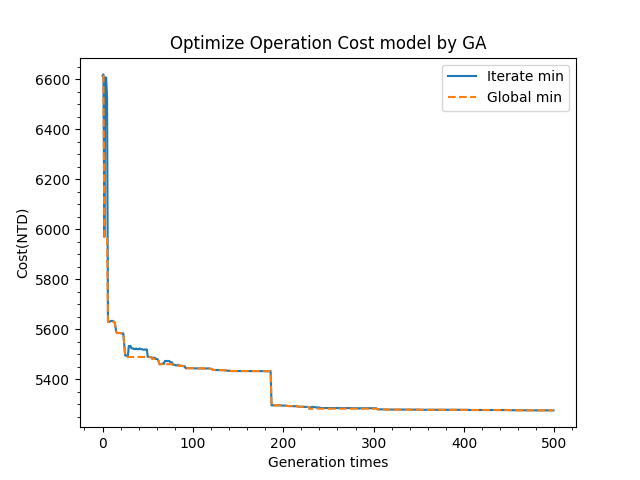
\includegraphics[width=8cm,height=6cm]{Graph/GAcost.png}
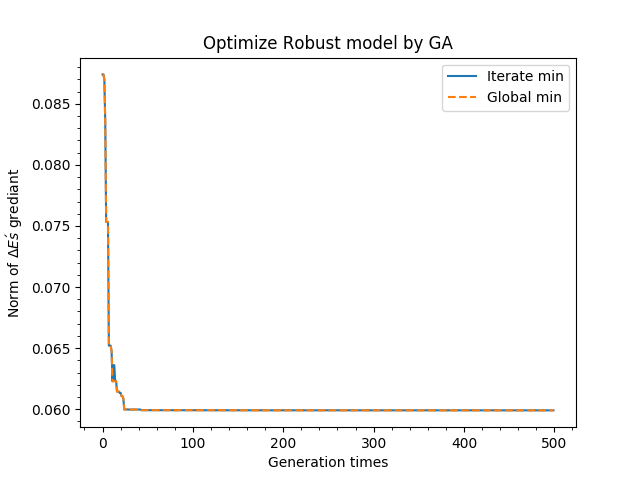
\includegraphics[width=8cm,height=6cm]{Graph/GARobust.png}
\center
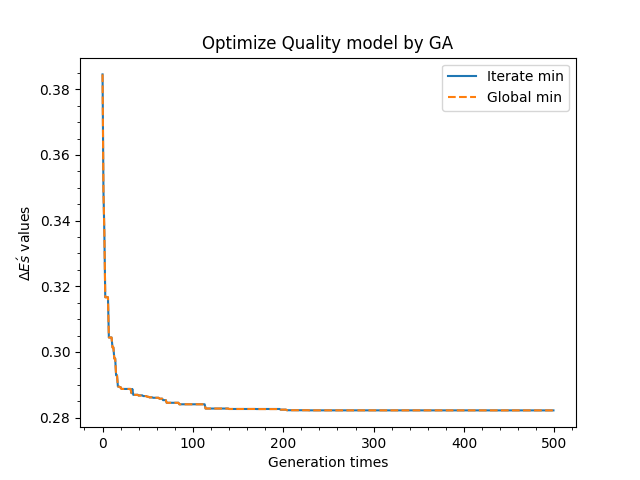
\includegraphics[width=8cm,height=6cm]{Graph/GADeltaE.png}
\caption{GA演算法搜尋各個模型最佳化收斂過程圖}
\label{fig:GAopt}
\end{figure}
\\由圖\ref{fig:GAopt}(左上)以GA演算法求解運作成本最小化模型,成本最佳解可以達到5275元,圖\ref{fig:GAopt}(右上)以GA演算法求解穩定度模型,其最佳解可達到約0.06,而圖\ref{fig:GAopt}(下)為品質成本的收斂過程圖,其$\Delta E$可達0.28,為了將得到的結果調整為符合實際紡織產業所能控制的範疇,如表\ref{tab:table7}將各個搜尋結果調整後分別套用至每個目標函數,便可比較製程參數組合間的差異。
\begin{table}[!htbp]
	\caption{基因演算法模型最佳化結果表}
	\center
	%!TEX root = ../thesis.tex
\begin{tabular}{ccccccccc}
\hline
\multirow{2}{*}{Items} &
\multicolumn{5}{c}{Factors} &
\multicolumn{3}{c}{\multirow{1}{*}{Result}} \\
\cline{2-9}
  & $x_A$ & $x_B$ & $x_C$ & $x_D$ & $x_E$ & Cost & Robust & $\Delta E$ \\
\hline\hline
最小化成本 & 51 & 1.3 & 76 & 18 & 15 & 5368 & 0.49 & 0.63 \\ 
穩定度最佳化 & 59 & 1.2 & 86 & 19 & 20 & 6590 & 0.065 & 0.168 \\ 
品質最佳化 & 61 & 1.2 & 82 & 19 & 23 & 7163 & 0.115 & 0.086 \\ 
\hline
\end{tabular}
	\label{tab:table7}
\end{table}





%!TEX root = ../thesis.tex
\section{最佳化參數組合與其他業界常用組合比較}
\label{c:ch6.4}
在這個小節當中,主要分別以本研究的最佳解方法以及可行範圍內隨機抽樣的樣本與業界常用的組合,相互比較並探討研究的方法在其他解中的優劣;在前面的小節,我們從模型數值化到序列二次規劃法以及基因演算法得到模型各自的最佳解與業界常用的組合,整理合併後得到表\ref{tab:table3}以及表\ref{tab:table7},但為了與其他可能會出現在業者所制定的染整製程參數組合比較,我們則從可行區域中提供幾組解作為比較的參數組合。
\begin{table}[!htbp]
	\caption{最佳化組合與其他業界常用組合比較表}
	\center
	%!TEX root = ../thesis.tex
\begin{tabular}{cccccccccc}
\hline
\multirow{2}{*}{Method} &
\multirow{2}{*}{Items} &
\multicolumn{5}{c}{Factors} &
\multicolumn{3}{c}{\multirow{1}{*}{Result}} \\
\cline{3-10}
  & &$x_A$ & $x_B$ & $x_C$ & $x_D$ & $x_E$ & Cost & Robust & $\Delta E$ \\
\hline\hline
GA演算法 & 最小化成本 & 51 & 1.3 & 76 & 18 & 15 & 5368 & 0.49 & 0.63 \\ 
& 穩定度最佳化 & 59 & 1.2 & 86 & 19 & 20 & 6590 & 0.065 & 0.168 \\ 
& 品質最佳化 & 61 & 1.2 & 82 & 19 & 23 & 7163 & 0.115 & 0.086 \\
\\
SQP方法 & 最小化成本 & 52 & 1.2 & 76 & 16 & 14 & 5044 & 0.558 & 0.775 \\ 
& 穩定度最佳化 & 59 & 1.2 & 86 & 18 & 20 & 6561 & 0.061 & 0.225 \\ 
& 品質最佳化 & 61 & 1.2 & 78 & 19 & 25 & 7545 & 0.255 & 0.042 \\ 
\\
隨機樣本 & 樣本一 & 54 & 1.4 & 79 & 14 & 22 & 6888 & 0.432 & 0.528 \\ 
& 樣本二 & 54 & 1.4 & 83 & 14 & 22 & 6975 & 0.285 & 0.557 \\ 
& 樣本三 & 54 & 1.4 & 83 & 16 & 22 & 7033 & 0.229 & 0.426 \\
& 樣本四 & 54 & 1.6 & 79 & 14 & 22 & 6888 & 0.399 & 0.611 \\ 
& 樣本五 & 54 & 1.6 & 79 & 16 & 22 & 6946 & 0.342 & 0.468 \\ 
& 樣本六 & 54 & 1.6 & 83 & 14 & 22 & 6975 & 0.254 & 0.609 \\ 
& 樣本七 & 54 & 1.6 & 83 & 16 & 22 & 7033 & 0.198 & 0.467 \\ 
\\
長期經驗 & 業界常用 & 56 & 1.5 & 81 & 15 & 20 & 6454 & 0.288 & 0.488 \\
\hline
\end{tabular}
	\label{tab:table8}
\end{table}

本研究以隨機抽樣的方式,搭配出不同的32種參數組合,但由於必須限制在$\Delta E$低於0.8以及$K/S$介於95到105之間,所以實際可行的隨機組合只有得到部分幾組,並將隨機的製程參數組合分別帶入各個目標函式後,如表\ref{tab:table8},將樣本的結果以及表\ref{tab:table3}和表\ref{tab:table7}合併後進行比較;從表\ref{tab:table8}可以觀察到,使用序列二次規劃法以及GA演算法搜尋的最佳解,在搜尋各自的項目上與其他的製程參數組合比較,是相對優秀的,說明此兩種方法在解決染整製程最佳化問題都能找到有效的區域最佳解;那麼在比較此兩種方法中,可以看出序列二次規劃法相對應的最佳化結果,都比基因演算法的結果再好一些,而且計算上更快速一些,故在表\ref{tab:table8}中,序列二次規劃法較基因演算法好一些,不過為了探討本研究提出的方法在整體上是否可以成功的替代業界常用的組合,我們必須從業界所提供的的其他資訊以及假設作為本研究整體評估的考量。

業界常用的製程參數組合,套用到實際的大染缸中,業者表示會有15\%的染布會與目標間存在差異,所以在$\Delta E$超過0.8時染布就需要重染或報廢,因此我們假設整體的報廢成本為失敗機率的等比級數總和乘以單次染布的運作成本,則我們假設評估整體的總成本為運作成本以及平均報廢成本的總和,而業界常用組合的平均總成本約為$6454\div (1-0.15)\simeq 7593$元。

業界常用參數是由長期的經驗法則所得來的結果,而且實際紡織業者提供一天所使用的染缸約160缸,故我們假設業界常用參數組合所呈現的$\Delta E$是符合平均數為0.488,及變異數未知的常態分配假設,雖然變異數未知,但我們從業者提供的資訊知道當超過$\Delta E$為0.8時,則失敗率為0.15中可推得其變異數為$[(0.8-0.488)/1.04]^2 = 0.09$;同樣的在這裡我們也假設其他的製程參數組合也符合平均數為各自的$\Delta E$,變異數為未知的常態分配,且通常越穩定的製程參數其$\Delta E$的變異會越小,故在這裡我們假設製程參數的變異數比與穩定度是成一般反比的關係,由以上這些假設條件下,我們便可以得到各組合的總成本,如表\ref{tab:table9}所示。
\newpage
\begin{table}
	\caption{最佳化組合與其他業界常用組合估計總成本比較表}
	\center
	%!TEX root = ../thesis.tex
\begin{tabular}{cccccc}
\hline
\multirow{2}{*}{Method}&
\multirow{2}{*}{Items} &
\multicolumn{4}{c}{Result} \\
\cline{3-6}
 & & Average & Variance & Failure rate & Total cost \\
\hline\hline
GA演算法 & 最小化成本 & 0.63 & 0.153 & 33.2\% & 8036 \\ 
& 穩定度最佳化 & 0.168 & 0.020 & 0.0005\% & 6590 \\ 
& 品質最佳化 & 0.086 & 0.036 & 0.0083\% & 7164 \\ 
\\
 SQP方法 & 最小化成本 & 0.775 & 0.174 & 48.0\% & 9700 \\ 
& 穩定度最佳化 & 0.225 & 0.019 & 0.0016\% & 6561 \\ 
& 品質最佳化 & 0.042 & 0.079 & 0.36\% & 7572 \\ 
\\
隨機樣本 & 樣本一 & 0.528 & 0.135 & 22.9\% & 8933\\ 
& 樣本二 & 0.557 & 0.089 & 20.7\% & 8795 \\ 
& 樣本三 & 0.426 & 0.072 & 8.1\% & 7652 \\
& 樣本四 & 0.611 & 0.125 & 29.6\% & 9784 \\ 
& 樣本五 & 0.468 & 0.107 & 15.5\% & 8220 \\ 
& 樣本六 & 0.609 & 0.079 & 24.9\% & 9287 \\ 
& 樣本七 & 0.467 & 0.062 & 9.0\% & 7728 \\ 
\\
長期經驗 & 業界常用 & 0.488 & 0.09 & 15\% & 7593 \\
\hline
\end{tabular}
	\label{tab:table9}
\end{table}

從表\ref{tab:table9}中,雖然隨機樣本的參數組合中的樣本三對業界常用組合較為穩定以及品質較高,但單次估計總成本卻比較高,可見業界常用組合是普遍在其他隨機樣本中確實是比較好的,而本研究的穩定度最佳化參數組合,以及使用基因演算法中的穩定度最佳化組合,則在估計總成本中比業界常用成本更低;雖然基因演算法穩定度結果與本研究方法差異不大,但是從綜合成本可量下,可看出本研究的方法還是稍微好一些,故在本研究的方法估計的綜合考量下,運作成本最佳組合以及品質最佳組合,雖然以該項目作為比較依據都比基因演算法好,但綜合評估下的成本卻比較高一些,故在選擇上業者需要自行評估哪一個模型比較符合當下需求,就本研究來說,建議使用SQP得到的穩定度模型最佳解是最好的選擇。

% \input{Chapter_6/section5}
% \input{Chapter_6/section6}
% Chapter 7
%!TEX root = ../thesis.tex
\chapter{結論}
\label{c:con}
本研究主要探討染色製程最佳化問題,從大略介紹機能布料對於現今世界的發展性,進而討論藉由降低紡織業在染色過程中的成本,提高紡織產業的利潤;為了有效降製程成本,我們數次拜訪業者,並由化驗室得來的實驗數據進行多項分析後,最後我們使用了五個對於染色過程中具有較大影響力的五個染整製程因子,作為本研究建置模型的決策變數,並根據這些製程參數的特性分別建置運作成本最小化模型、穩定度模型以及品質模型($\Delta E$模型),並藉由序列二次規劃法作為本研究的最佳化方法,分別對三個模型搜尋最佳解,因此分別得到模型的製程參數最佳組合;在數據分析中我們將其他文獻所使用的方法做為比較的對象,以基因演算法針對本研究的三個模型分別求解,得到的製程參數組合做為對照組合,另外我們還從可行區域內隨機抽取其他製程參數組合,最後將所有的製程參數組合與業界常用的組合互相比較。

在數據分析,在我們的假設下得知,序列二次規劃法中的穩定度最佳化模型所求得的製程參數組合,與其他的製程參數組合互相比較下,品質較好且較為穩定且所需要花費的運作成本差異不大,如果以每年250個工作天以及每天需要染整160缸染布下,約可以節省報廢或重染成本約每年三千多萬台幣,對於業者來說是相當可觀的成本花費。

本研究中主要只有探討五個具有顯著的影響成本、品質,以及業者有興趣的製程參數,並且根據運作成本以及品質進行求解以及數值分析,但實際的染整製成參數多達數十種,如在未來有機會能夠再與業者合作,可增加製程參數的種類以及增加實際現場的實驗數據,增加模型的可信度,並可以導入成本導向以及品質導向的目標合併,如多目標方法,在多製程參數下求取成本以及品質之間的最佳平衡點,除了為業者減少報廢成本外還能有效降低其他的成本。

\appendix
\backmatter
%參考文獻
\renewcommand\bibname{參考文獻}
%\addcontentsline{toc}{chapter}{\bibname}
% \bibliographystyle{abbrv}
\bibliographystyle{apacite}
\bibliography{thesis}
\end{document}
